\documentclass{article}
\usepackage[utf8]{inputenc}
\setlength{\parskip}{1em}
\usepackage{subcaption}
\usepackage[table,xcdraw]{xcolor}


\title{Chapter 2}
\author{Jonathan S. Abrahams }
\date{October 2019}

\usepackage{natbib}
\usepackage{graphicx}
\usepackage{multirow}
\usepackage{graphicx}
\begin{document}

\maketitle

\section{Introduction}
%To do:
%1. sequencing stat for other datasets
%2. Table of 8 reads results?
%3. Blast some of these junction sequences from assembly graph and compare to basketball
%4. Synthesise an overarching argument for chapter 1 and 2
%5.
It was established that read depth can be exploited as a reliable proxy to find copy number variants in Chapter 1. There was, however, an inconsistency in the dataset: Copy number predictions were frequently not integers. 

In polyploid organisms it is often expected to observe non-integer copy number changes: a duplication of just one copy of a gene in a diploid organism, an overall change from 2 copies to 3 copies, would be estimated as a CNV with copy number 1.5. In bacteria, however, the interpretation is much less straightforward. In this chapter I investigated the basis for mixed copy numbers. In addition I aimed to resolve tandem duplications in BP.

\section{Results}

\subsection{Indication in short read data of mixed populations}



Intermediate copy number estimates were most recognisable in the dataset of 25 manually resolved genomes. The graph of copy number inconsistencies is replicated here (Figure \ref{fig:CDC_breakpoint} ). The discrepancy between the estimated copy number and the resolved copy number was evident as 52\% (13/25) strains had a copy number that differed by at least 0.3. 




\begin{figure}[h!]
\centering
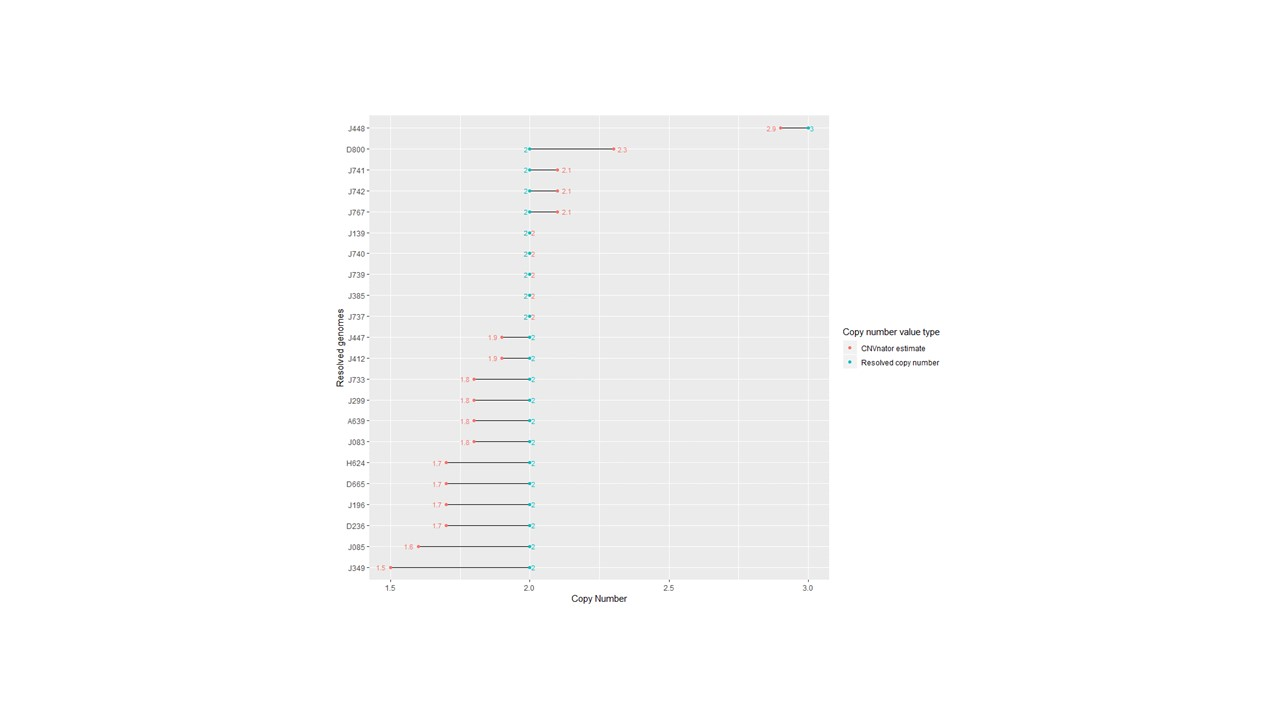
\includegraphics[width=\textwidth{}]{Chapter_1/copy number comparison.jpg}
\caption{ Copy number discrepancies between the Resolved copy number (blue) and the read depth based prediction (orange) (Reproduced from Chapter 1)}
\label{fig:CDC_discrep}
\end{figure}


A similar trend was also observed in the 278 CNVs predicted in the global cohort of ~2700 Bordetella pertussis strains. Although the true copy numbers of these isolates were not known. In this case, the prevalence of  intermediate copy number estimates that were +/- 0.3 of an integer in the full cohort of 278 CNVs was 71\% (193/272).
\begin{figure}[h!]
\centering
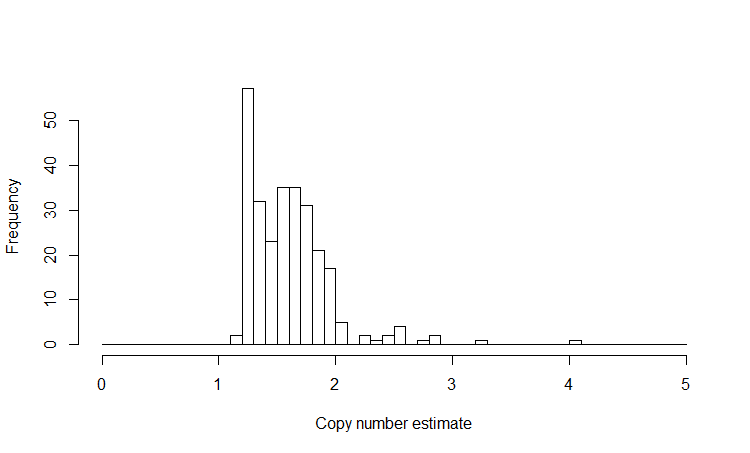
\includegraphics[width=\textwidth{}]{Chapter_2/Rplot.png}
\caption{ Copy numbers of }
\label{fig:Full_data_discrep}
\end{figure}

A technical artefact or combination of artefacts could have been the source of such a pattern, for example: uncorrected sequencing bias; bioinformatic analysis or sample preparation. Alternatively, however, this pattern could be produced, at least in part, by a biological source.

%https://www.ncbi.nlm.nih.gov/pmc/articles/PMC149199/pdf/gkg178.pdf

It is hoped, in most sequencing applications, that all cells in the population are clonally derived and have identical genomes. This leads to an easy to analyse genome during the assembly stage: all reads (derived from a number of different cells in the population) will contain the same DNA sequence differing only by sequencing errors. Whilst ideal, this scenario is not often acheived as some mutation types occur so frequently that within just a few generations, either within the host or in-vitro after isolation, variation between clonally derived cells is generated. Most of these mutations are small and inaccuracy in their exact composition  is well tolerated for msot applications. The best known example is slip-strand mutations in homopolymeric tracts- these mutations can occur as frequently as 1.5 -\^ 3 10\^-2. Copy number variants are also a mutation type that occurs very frequently, far more frequently than SNPs. It was therefore possible that the intermediate copy numbers observed in the dataset were products of cell to cell variation in copy number-either occuring before (in-vivo) or after (in-vitro) isolation of the sample. 
 


\subsection{Nanopore sequencing confirms mixed populations}

\subsubsection{Resolving duplications to find cell to cell differences}
In order to understand if mixed populations of cells were driving intermediate copy number estimates in BP it was necessary to resolve duplications using single DNA molecules using long read sequencing. 

It was hypothesised that if reads could be sequenced that were longer than a CNV in its tandem array then cell to cell differences could be studied. For example, if two reads were found to span the entire CNV locus including the single copy flanking regions, but each read contained a different copy number of the locus it could therefore be deduced there was at least two genotypes in that population. The most parsimonious explanation of such a result is that the two reads came from different cells, each with a different copy number. In this way, long read sequencing can be used to investigate cell-cell differences in copy number.

Whilst Long read sequencing on the PacBio platform has been undertaken to resolve duplications in BP previously, it has only been possible in combination with optical maps (which produce DNA fragments 50-750kb long) as a guide. The short read length of Illumina data or the limited length of PacBio reads (on average 10kb long), prohibits the study of CNVs as the reads are shorter than the CNV length. The Nanopore sequencing platform was therefore very attractive, as theoretically limitless length reads could capture a whole duplication in its tandem array (predicted to be 50kb to >600kb). 

BP isolates had previously been sequenced on the Nanopore platform using standard length reads and whilst this produced closed genomes, there was evidence that large duplications remain unresolved.

I therefore  investigated using ultra-long Nanopore reads in resolving long CNVs in B.pertussis  and in turn, investigating mixed populations of cells.

\subsubsection{Intermediate copy numbers in short read data linked to mixed populations in UK54}
To confirm our predictions from short-read sequencing data (Figure \ref{fig:Full_data_discrep} & Figure \ref{fig:CDC_discrep}) and investigate the basis for non-integer copy numbers, we exploited the tractable size of one relatively small CNV. The genome of UK54 (SAMEA1920853) was predicted to have a 16 kb CNV at a copy number of 4.1; short enough to observe the entire CNV locus in a single sequence read on the Nanopore platform, assuming that each copy occurred in tandem as observed in both our data and previous reports (refs). 

%protocol ref dx.doi.org/10.17504/protocols.io.mrxc57n
Ultra long DNA was prepared according to the Quick et al protocol. Whole genome sequencing on the Nanopore platform yielded 85k reads. This sample contained a low median and mean read length of only 1kb and 9.1kb  respectively,but produced over 3000 reads with a length exceeding 50kb. Sequence reads that contained both of the regions flanking the CNV locus and the CNV locus itself were identified (n = 9) and contained the CNV at different copy numbers (Figure 3). This demonstrated that a laboratory culture of UK54 comprised a mixture of copy numbers at this locus and explains the non-integer copy numbers predicted by the short read prediction pipeline. Genomic DNA for sequencing is derived from laboratory populations of bacteria and if these harbour CNVs at different copy numbers, subsequent read-depth based predictions will represent the average read depth of all of the bacteria sequenced.

Not all of the  sequencing characteristics of Nanopore runs are noted here. This initial ultra-long nanopore sequencing experiment,however, had a low yield of <100k reads with many reads being very short. Subsequent runs contained over 5x as many reads and with much higher median and mean lengths.


\begin{figure}[h!]
\centering
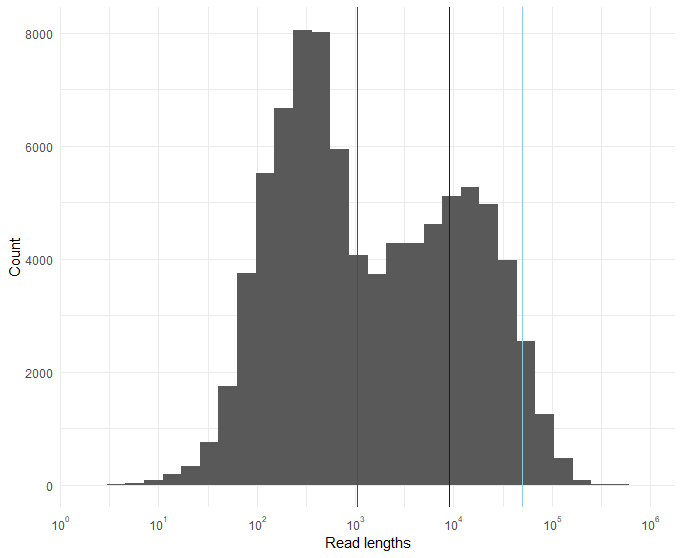
\includegraphics[width=\textwidth{}]{Chapter_2/read counts.png}
\caption{ Read length histogram for UK54. A median of 1kb (red line) and a mean of 9kb (blue line) were observed in addition to over 3000 reads exceeding 50kb in length (light blue line).}
\label{fig:Read_counts}
\end{figure}




\begin{figure}[h!]
\centering
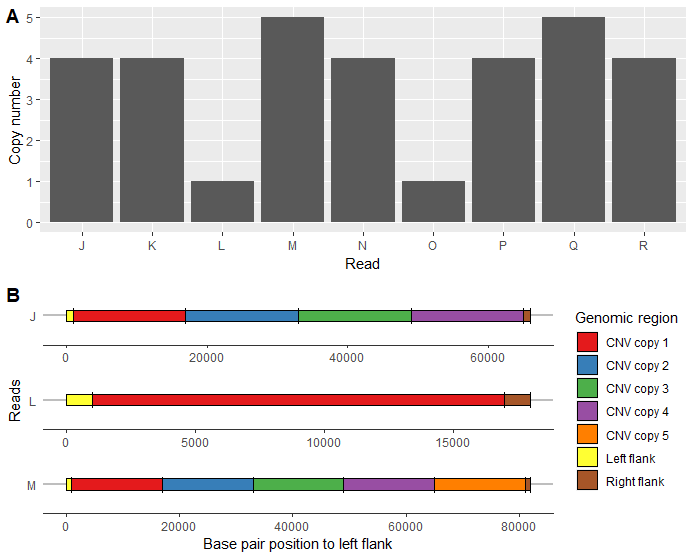
\includegraphics[width=\textwidth{}]{Chapter_2/combined UK54.png}
\caption{ Ultra-long read sequencing of UK54 revealed the presence of different copy number CNV loci within a single culture. Individual sequence reads that spanned the CNV loci were identified using Blastn, labelled J to R. (Panel A). The data shows each read (x-axis) containing 1,4 or 5 copies of the locus (y-axis) and therefore, as each read appears to be integrated into the chromosome, there were cells present in the population with 1, 4 or 5 copies of the locus. The arrangement of the relevant section of three reads (J, L and M) is illustrated in panel B.}
\label{fig:CDC_discrep}
\end{figure}
%https://assets.publishing.service.gov.uk/government/uploads/system/uploads/attachment_data/file/583859/Q_5i2.pdf
As official guidelines to medical microbiologists recommend to take "one or multiple" colonies from a plate when making liquid culture, it was not known if the original culture of UK54 involved isolation of a single colony or collection of multiple clones from the diagnostic plate growth. Thus it was unclear whether the observed variation in copy number resulted from a mixed culture or emerged during laboratory growth prior to sequencing.  To therefore definitively show that mixed populations can arise from clonally derived populations, single colonies were isolated.

%We can use these graphs to further confirm the short read predictions are actually bloody accurate. compare this data with expected counts, based on distribution of read lengths. Only do this if I am hard up for results!


\subsubsection{Mixed populations from pure cultures}
To investigate mixed populations, IM picked eight single colonies of UK54 and passaged them once by growth on agar and then once during broth growth. Each of these clonal populations were theoretically derived from a single bacterium. The copy number at the CNV locus in each of the resulting clones was estimated using qPCR (Figure \ref{fig:8_clones}) and ranged from 2.2 (clone 6) to 51.2 (clone 8). This experiment therefore demonstrated that the original UK54 population was a mixture of cells with different copy numbers. The results were not conclusive in regards to how this variation was generated however and the question still remained: were CNVs unstable over very short timescales (<30 generations)?.


\begin{figure}[h!]
\centering
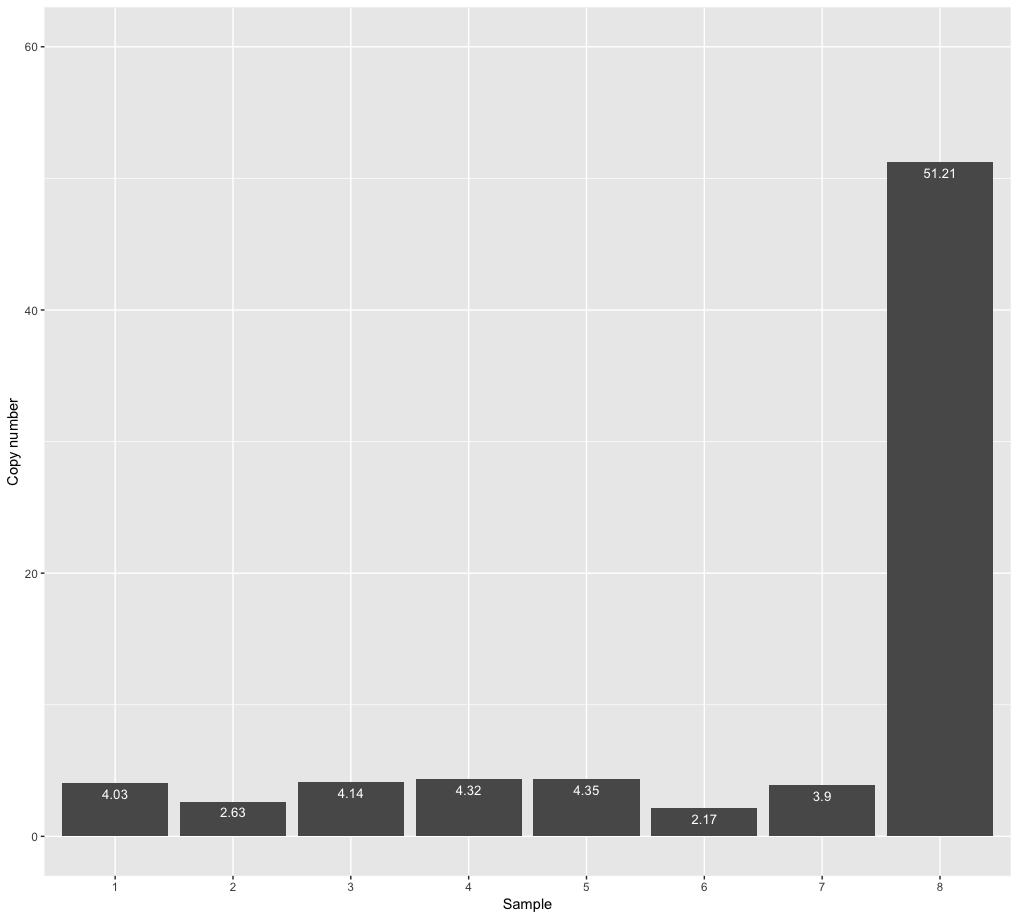
\includegraphics[width=\textwidth{}]{Chapter_2/8 clones.png}
\caption{ Quantification of CNV copy number of 8 clones of UK54 by qPCR demonstrated a range of copy numbers from 2.17 to 51.21}
\label{fig:8_clones}
\end{figure}

Seven of the 8 clones had expected copy numbers of between 1 and 4, but clone 8 had an unexpectedly high copy number. Whilst a copy number of 51 may seem improbable from a population which has an average copy number of 4, it is known that tandem duplications are highly unstable and prone to further amplification This is expanded on in the discussion.

In order to demonstrate the highly unstable dynamics of CNVs, two of the UK54 clones which had a range of copy numbers of the locus from 4.3 copies to 51.2 copies were sequenced using the ultra-long nanopore protocol. It was hypothesised that as these samples were clonally derived each sample should, if copy number was not plastic over short time scales (the null hypothesis), contain reads containing the CNV locus at the same copy number. The same BLAST search method was applied as previously.

\begin{figure}[h!]
\centering
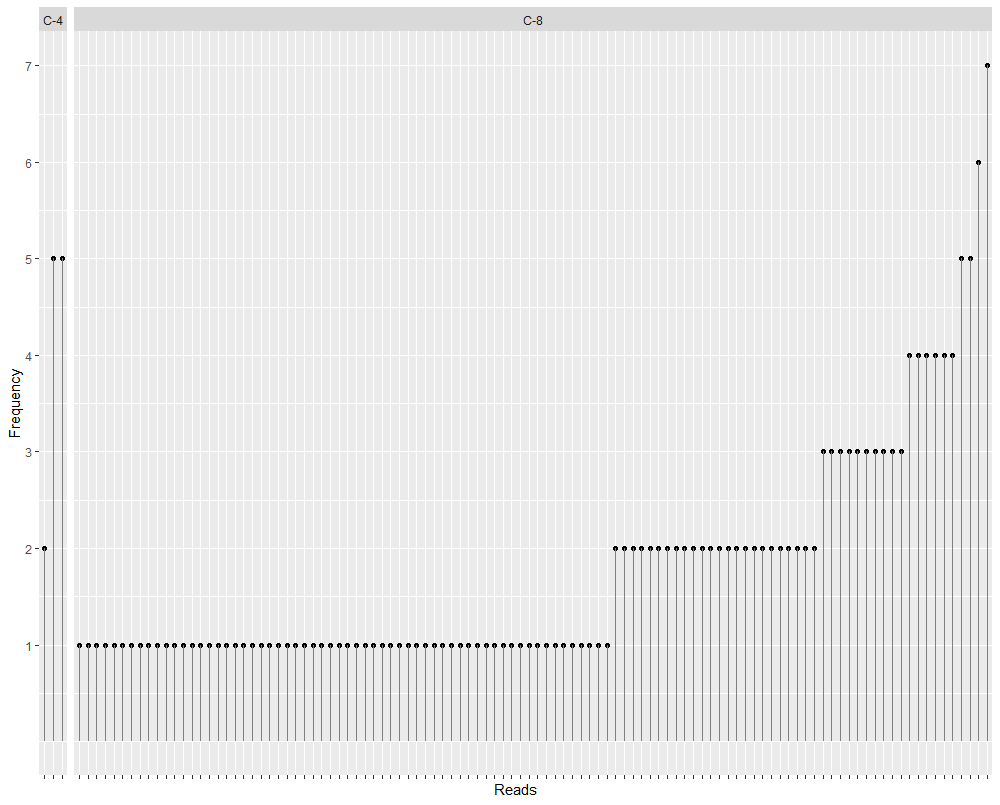
\includegraphics[width=\textwidth{}]{Chapter_2/clone 4 and 8.png}
\caption{ Ultra-long read sequencing of UK54 clone 4 and 8 (C-4 and C-8) revealed the presence of different copy number CNV loci within a single culture. Individual sequence reads that spanned the CNV loci were identified using Blastn successfully in clone 4 whilst clone 8 had no reads spanning the full locus. Therefore partial reads were plotted for clone 8. The data shows each read (X axis) contained between one and seven copies of the locus (Y axis).}
\label{fig:Clone_4_8_reads}
\end{figure}

The isolate UK54 clone 4 was sequenced using the Nanopore platform and sequence reads were observed with copy numbers  2 and 5 (Figure \ref{fig:Clone_4_8_reads}). These data strongly suggested that CNV copy number was plastic, with copy number variants arising during in vitro growth from a single bacterium to the culture from which the gDNA was extracted. 

%It was interesting to note that the qPCR screening results agreed completely with the depth of coverage (generated on the Nanopore platform) of the CNV loci in all three isolates, cementing qPCR as an effective screening tool to identify CNV copy number.

Taking these results (Figure \ref{fig:8_clones} \& Figure \ref{fig:Clone_4_8_reads}) as a whole it is clear that for isolates with a CNV, copy number change is a dynamic,fluid and continual process in Bordetella pertussis.

Nanopore sequencing was also performed with UK54 clone 8, which qPCR showed to have  a copy number of 51 by qPCR (corresponding to a predicted CNV length of 816kb) (Figure \ref{fig:Clone_4_8_reads}). No reads spanning the entire CNV locus (i.e. the CNV locus with single copy flanking DNA on each side) were produced, presumably due to its extreme length. However, reads containing up to 7 copies of the locus, without flanking regions, were identified. Relaxing the Blastn alignment parameters from a 90\% minimum query length of the CNV locus to 50\% identified a maximum of 9 copies of the locus present on a single read with incompletely sequenced copies at each end. Consistent with the copy number prediction from qPCR, the read depth at this locus for UK54 clone 8 from the Nanopore data was approximately 60x higher than the genome average, strongly supporting the very high copy number estimate for this locus in this clone.

\subsubsection{Expression is linked to copy number}

To investigate potential phenotypic variation resulting from amplification of genes by CNV formation, IM measured mRNA levels for one gene within the CNV locus in three UK54 clones. We selected clones 2, 4, and 8, with originally screened copy numbers of 2.63, 4.32, and 51.21, respectively. RNA expression of gene X was normalized to the single copy gene recA, an often used as a stably-expressed housekeeping gene in RT-qPCR experiments.

As we demonstrated that each culture comprises a heterogenous mixture of cells with varied CNV copy number, we re-eassayed the locus copy number for each clone using the same laboratory culture from which RNA was extracted. Upon re-growing these clones for RNA extraction, the average copy number in each changed (statistically non-significantly) to 4.1, 6.5, and 53.1 in clones 2, 4, and 8, respectively.

The mRNA level for the gene X (contained within the CNV) corresponded with the copy number (Figure 6); normalising the transcript level in clone 2 to a value of 1, it was 16.8 fold higher (P<0.0001) in clone 8. It was also higher, but not significantly, in clone 4 (P=0.76). However, broadly, using the data as a whole, there was an association between DNA copy number and transcript abundance. This strongly suggests that the CNV altered gene dosages  effected relative gene expression levels.

\begin{figure}[h!]
\centering
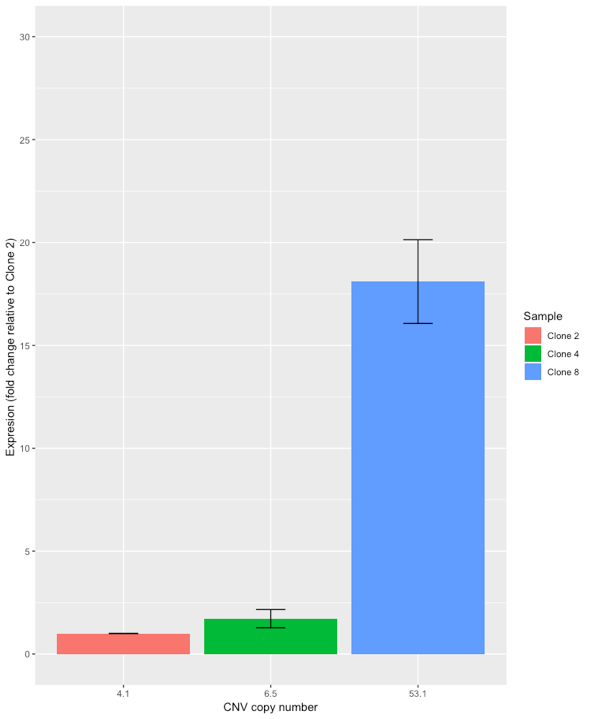
\includegraphics[width=\textwidth{}]{Chapter_2/DNA RNA.png}
\caption{  Copy numbers of clones 2, 4 and 8 were quantified using qPCR and expression of a gene within the CNVs was quantified by RT-qPCR. Expression is shown as a relative fold change to Clone 2. Error bars represent standard deviation of expression. The results show that copy number corresponds to RNA expression.}
\label{fig:Clone_4_8_reads}
\end{figure}


\subsection{Structural variants in Nanopore reads with no prior information}

Analysing the Nanopore data from clonally derived populations strongly suggested that the CNV locus in UK54 was plastic, leading clonal populations to quickly diversify. These analysis and experiments, however, only studied one specific locus- the locus that was predicted to change. It was possible that using a more agnostic method of identifying reads containing SVs, other loci around the genome were also undergoing structural variation at much lower rates. I explored this hypothesis in order to generate further insights into genome dynamics of BP.


\subsubsection{Naive identification of SV events in single reads}

To investigate if other loci around the genome underwent SV during in-vitro culture, sequence reads that contained sequences which were proximal on the read read but distant on the consensus genome sequence were found. These were putative structural variants. 

Each read was compared to the  consensus sequence  using a BLAST search. This was technically very challenging as this process was frustrated by the high repeat content of BP. Any time a repeat sequence was found, it was a technical hurdle to decide if there was a sequence was following the repeat that would be expected or if there was an unexpected sequence (indeicating a SV). To overcome this efficiently, it was necessary to remove the repeat gene content from the BP genome. The genome was split up into 1kb window at a step of 200bp and any 1kb section that appeared more than once with adeqaute homology in at least 50\% of the length of the window was deleted. For UK54 this removed 2Mb of sequence giving a consensus sequence length of 3.5Mb. Whilst this was highly conservative it aided efficient and accurate analysis of reads.

After homology searching against the repeat-depleted consensus sequence, any read which contained two adjacent parts DNA sequences that mapped to two different parts of the genome (separated by at least 30kb in order to avoid picking up stretches of bad quality sequence) was isolated. As all observed CNVs in pertussis appear to have been formed by homologous recombination between genes with multiple copies, this was a clear marker for CNVs. In order to ascertain if the junction sequences were in repeat elements, despite each read being compared to a consensus sequence depleted of repeat elements, these reads were then compared to the full consensus sequence. Only the reads which appeared to have junctions between disparate sequences on the genome in repeat regions (within 1kb) were kept. This resulted in 29 reads in this analysis.

As this plot resembled a basketball, I therefore named this whole analysis (from identifying single reads with SVs to plotting) a basketball analysis.


\begin{figure}[h!]
\centering
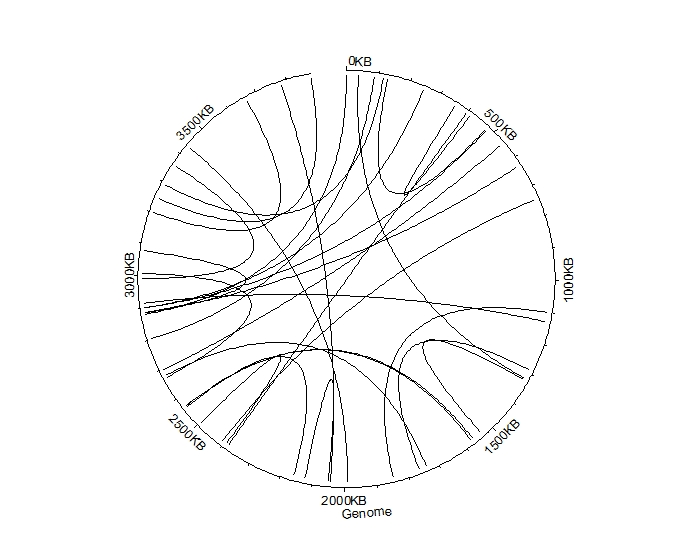
\includegraphics[width=\textwidth{}]{Chapter_2/Circos_Naive.jpeg}
\caption{A circos plot with all the 29 reads found to have juxtaposed genome positions. Lines join the two regions of the depleted genome that were proximal on the read but distant on the genome.}
\label{fig:Junc_proximity}
\end{figure}

It is naive, however, to assume that all of these reads are true SVs. It is possible that they are sequencing errors. Such errors have a characteristic appearance,however. In order to verify these results, the  hypothesis that at least some of these reads are chimeras was thoroughly investigated.

\subsubsection{How do sequence errors appear?}
%THis paper has fantastic references to investigate how many non-IS flanked duplicated should be observed.
%https://www.ncbi.nlm.nih.gov/pmc/articles/PMC4315931/
It is possible that adapter sequences can be ligated to two DNA fragments on either side, effectively joining together two random parts of the genome and thus, when sequenced, appearing as a structural variation. It is also possible that two separate reads can pass through the pore in quick succession, leading them to be classed as a single read. These two sources of erronous reads are known as chimeric reads. Some studies have estimated chimera formation happens at a rate of upto 2\% during Nanopore sequencing, although this may depend on if a ligase enzyme is used in the library preparation, which was not the case here.
 
There are three traits of SVs that allow them to be distinguished from chimeric reads: Long length; association with repeats and gapless junctions. This means these characteristic hallmarks are rare to appear in combination by chance in sequence data. This is in contrast to SNPs which,due to their comparitavely simple nature, are  impossible to tell the difference between a true SNP and a sequencing error- there is simply not enough information.  It is therefore theoretically possible to distinguish between a SV and a sequencing error in a single read. This proved key to studying sub-populations of cells. 
 
As adapter sequences are synthetic DNA that is added to the sequencing reaction and does not occur in the BP genome, I hypothesise that when each read was blasted against the consensus sequence the chimeric reads will have a gap in sequence homology to the reference and that within this gap an adapter sequence may be found.

\subsubsection{Gaps in alignments indicate chimeric DNA}
Analysing the blast results, three main types of reads were found: reads with junctions in close proximity (Figure \ref{fig:Junc_proximity} (but not immediately adjacent) to repeats; Reads with gaps immediately adjacent to a repeat element (Figure \ref{fig:Gap_adj}) and Gapless reads (Figure \ref{fig:Gapless}). The basketball plot was modified to reflect these categories (Figure \ref{fig:Basketball_3_errors}).

\begin{figure}[h!]
\centering
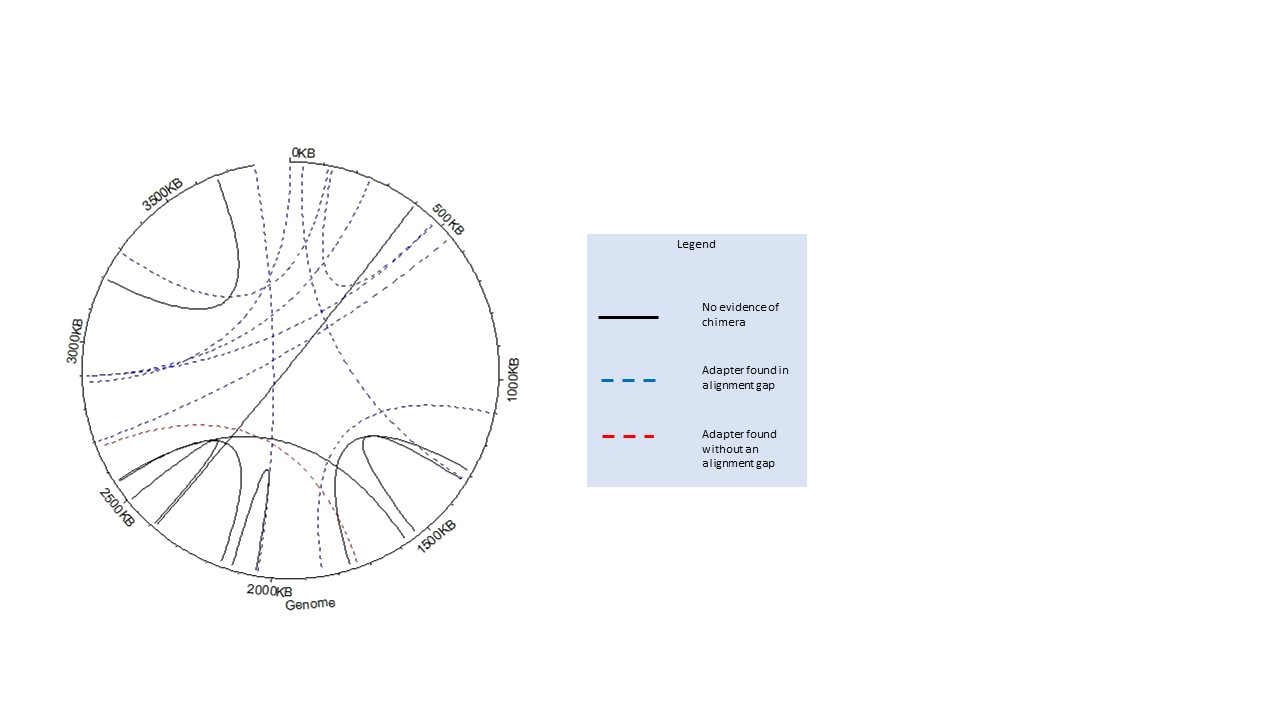
\includegraphics[width=\textwidth{}]{Chapter_2/baskey [Autosaved].jpg}
\caption{A basketball plot of the three main types of reads identified in this analysis. }
\label{fig:Basketball_3_errors}
\end{figure}

%reads with junctions in close proximity graph
It was found that 9 reads were found to contain junctions (with or without gaps) in close proximity, but not directly adjacent to, repeats. Reads with junctions in close proximity are likely identified in this experiment because I selected reads in which the junction occurred within 1.5kb up or downstream of an insertion sequence. These reads may infact indicate CNVs arising from NHEJ or chimeric reads. They were analysed for adapter sequences and then excluded from further analysis (see section x).


\begin{figure}[h!]
\centering
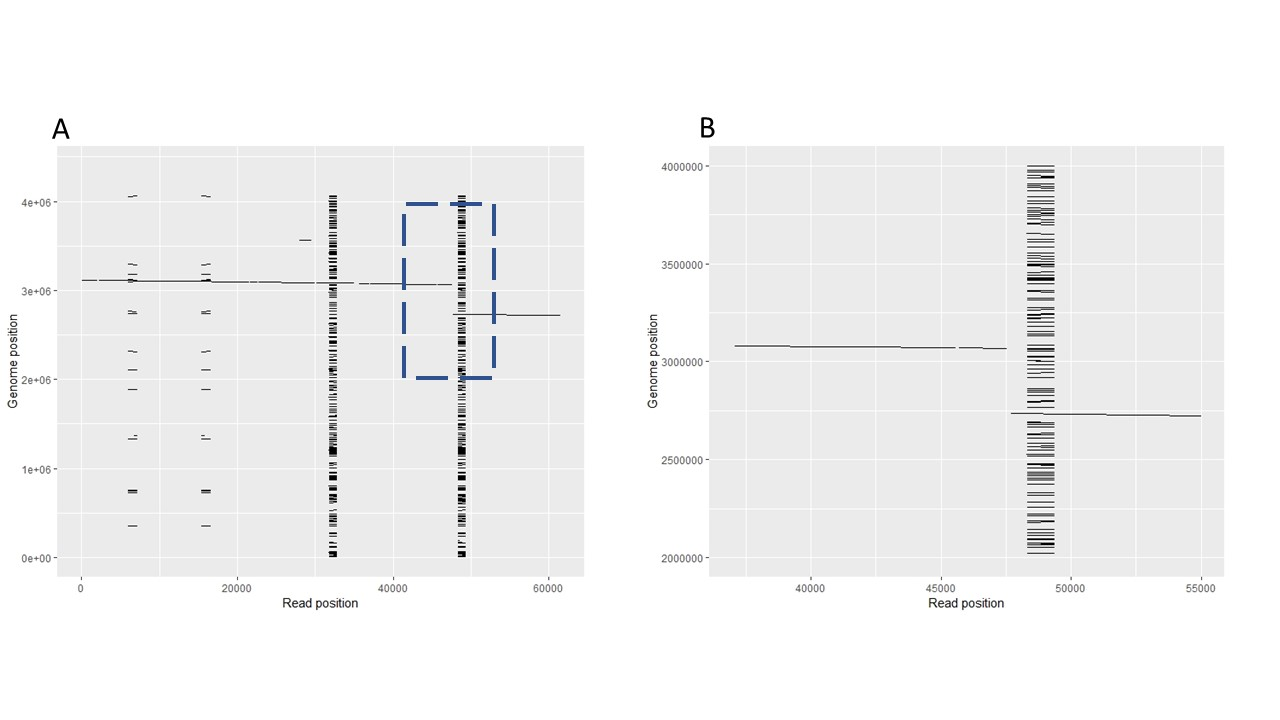
\includegraphics[width=\textwidth{}]{Chapter_2/odd read.jpg}
\caption{A read which did contained a gap following a repeat element, in this case a 3kb sequence which has two copies in distant parts of the genome.}
\label{fig:Junc_proximity}
\end{figure}

Reads with gaps immediately adjacent to a repeat sequence are likely to be chimeras, based on the hypothesis that an adapter sequence would cause a gap in an alignment.

%Reads with gaps immediately adjacent to a repeat element 
\begin{figure}[h!]
\centering
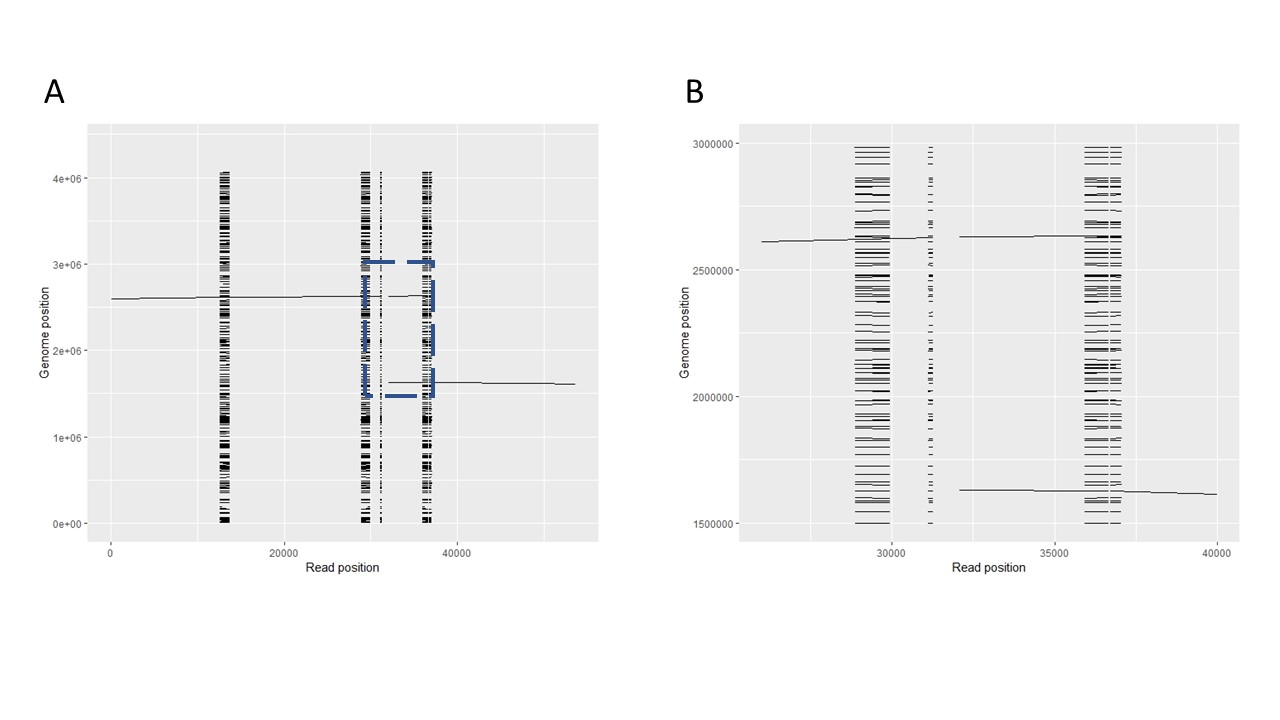
\includegraphics[width=\textwidth{}]{Chapter_2/Gappy read.jpg}
\caption{A read which did contained a gap following a repeat element, in this case a 3kb sequence which has two copies in distant parts of the genome.}
\label{fig:Gap_adj}
\end{figure}


%Gapless reads

A number of reads appeared with no gap in the sequence alignment. I hypothesise that these reads are true SVs that have occurred during brief culturing.
\begin{figure}[h!]
\centering
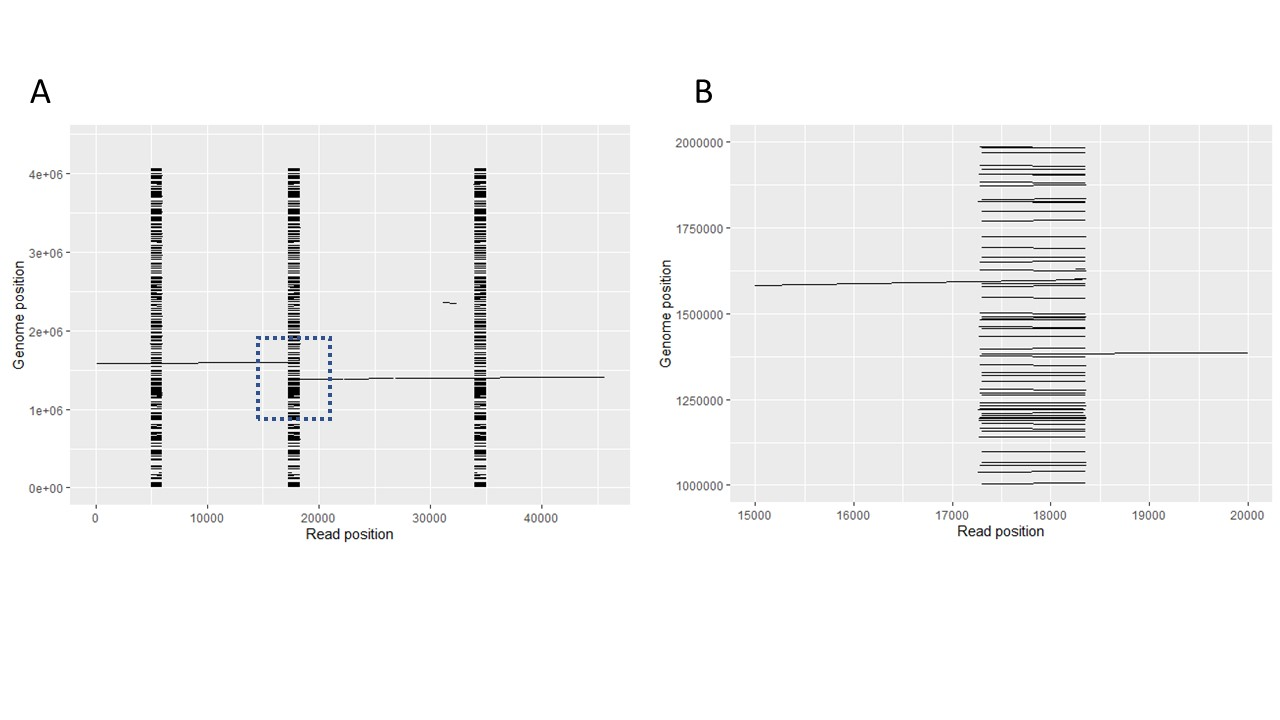
\includegraphics[width=\textwidth{}]{Chapter_2/Read 9(2).jpg}
\caption{An exemplary read which did not contain any gaps gaps in  the read and consensus sequence alignment.}
\label{fig:Gapless}
\end{figure}



Whilst gaps indicate that a read might be a chimera, the presence of an adapter sequence in this gap is unequivocal evidence of this. Adapter sequence searching,however, is complicated by the inherent raw error rate of Nanopore reads which, for the chemistry used here, results in approximately 75-90\% accurate reads. It was therefore necessary to identify not only containing the perfect adapter sequence, but sequences that were similar to the adapter sequence- a fraught process.

\subsubsection{Inexact string matching is hard on error prone data}
%Potentially need to switch the simulation data from simulated data to the ligation made French isolate. To simulate chimeras I can take random 1kb stretches from this data and jam them together with adapters.

As DNA is composed of a 4 letter alphabet, two random sequences can match with approximately 50\% homology (see \ref{fig:Histo_homo}. Therefore, identifying sections of DNA that have are approximately 60-80\% similar to their true sequence is a technical challenge.

In order to demonstrate how challenging this process is, 2k true negatives (random sequences with gc content of 67\%-same as pertussis) were simulated and true positives taken from the first 100bp of 2k UK54 clone 4reads. These DNA segments were aligned to the adapter and the percentage homology plotted. The results show that in order to recognise 99\% of adapter sequences in this dataset it would be necessary to allow homology matching down to 50\% homology which has a false positive rate of 34\% in the test scenario. However, If only 90\% of the chimeras were to be excluded then adapter homology threshold could be set to 76\%, leading to a false positive rate of X. How this would impact the UK54 dataset is worked through in Table \ref{tab:Homo_example} on an estimation that chimeras are formed at a rate of 2\%

Conducting a simulated analysis on adapter sequence matching demonstrated how easily false positives are generated when inexact string matching is undertaken on error prone reads. I sought to find reads with adjacent DNA sequences that mapped to distant parts of the consensus sequence, a process that would also highlight many chimeras. Therefore in order to increase the confidence in my dataset, I needed a more stringent method to remove chimeric reads. 
 

%I need to run a simulation of chimeric reads: 2k reads with an adapter in the middle and 2k reads with

\begin{figure}[h!]
\centering
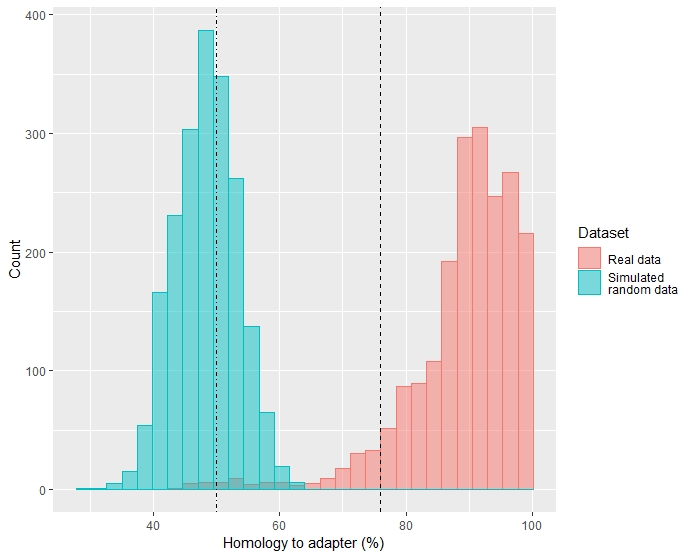
\includegraphics[width=\textwidth{}]{Chapter_2/Rplot01.jpeg}
\caption{A histogram of adapter homology search results in real data containing adapters and simulated data which did not contain adapters. The threshold that would remove 90\% of chimeras (76\% homology) is indicated with a dashed line and the threshold that would remove 99\% of chimeras is indicated with a dash-dot line. }
\label{fig:Histo_homo}
\end{figure}

\begin{table}[]
\resizebox{\textwidth}{!} & 99.00\% & 56.00\% & $\sim$14k & 140 \\ \cline{4-7} 
 &  &  & 90.00\% & 76.00\% & x & 1400 \\ \hline

\end{tabular}%
}
\caption{A table of worked examples of chimera matching based on the UK54 clone 4 dataset}
\label{tab:Homo_example}
\end{table}

\subsubsection{Searching for adapters within alignment gaps effectively identifies chimeras}

There were 9 reads that were selected by this analysis as having junction sequences within 1.5kb of an repeat element. As a broad search was conducted to find reads close to repeat elements but only the reads which have junctions fully adjacent to repeats was required, these 9 reads were excluded. However, under the assumption that homologous recombination between repeat genes is the primary source of SVs, it was hypothesised that these reads were chimeras. In agreement with this,  7 out of these 9 reads contained an adapter sequence at the sequence gap. This indicated they were chimeras rather than true SVs caused by non-homologous recombination or homologous recombination between small repeats. Excluding these 9 reads from the 29 reads left 20 reads which had junctions directly adjacent to repeat elements.


As expected, gaps in sequence alignment were often due to adapter sequences being present (Table \ref{tab:Adapter_Summary}). This provided evidence that in order to exclude chimeras with the highest stringency, an additional search rule should be added: reads which contained gaps directly adjacent to junctions in their alignment to the consensus sequence should be excluded. 

Therefore in summary these are the rules which were adhered to in order to highlight reads as true SVs:

\begin{enumerate}
\item Contains DNA sequences which are proximal on the read but at least >30kb apart on the consensus sequence, forming a `junction sequence'
\item The junction sequence must be directly in or adjacent to a repeat region
\item There must be no gaps in homology between the read and the consensus sequence adjacent to the junction sequence
\end{enumerate}


Following these search parameters left 8 reads which passed all tests and had no evidence that they were chimeras. I hypothesise that these are structural variants. 

\begin{figure}[h!]
\centering
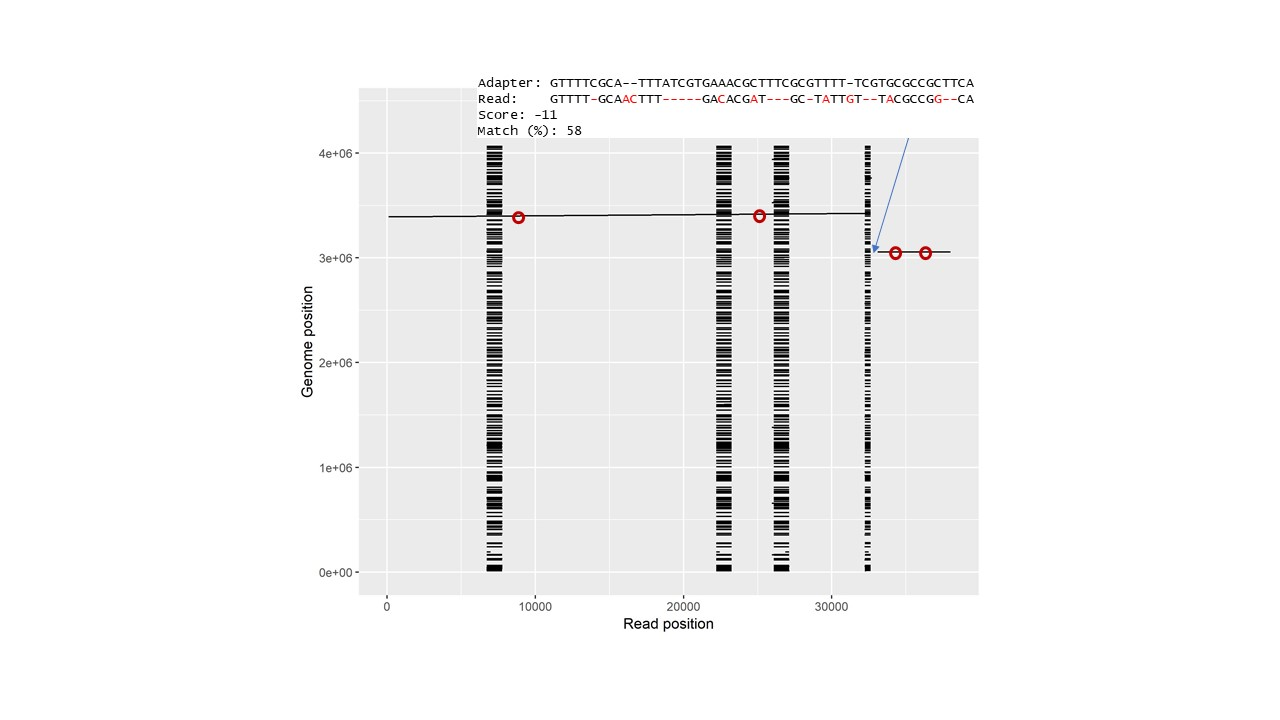
\includegraphics[width=\textwidth{}]{Chapter_2/Adapter read1123.jpg}
\caption{A read with a gap in sequence homology between the read and the consensus sequence. An adapter was found here with 58\% homology to the true adapter sequence. The alignment of the adapter to the found sequence is shown and differences are highlighted red. }
\label{fig:Adapter_in_gap}
\end{figure}

\begin{table}[]
\resizebox{\textwidth}{!}{%
\begin{tabular}{|l|l|l|l|}
\hline
Read category & Number of reads & Number with detectable adapter & Number without adapter \\ \hline
Junction not adjacent & 9 & 7 & 2 \\ \hline
Adjacent with gaps & 11 & 9 & 2 \\ \hline
Adjacent without gaps & 9 & 1 & \cellcolor[HTML]{FCFF2F}8 \\ \hline
\end{tabular}%
}
\caption{Table outlining the categories reads were placed into and how many adapter sequences were found. The 8 reads which passed all filtering are highlighted in yellow.}
\label{tab:Adapter_Summary}
\end{table}



\subsubsection{High confidence reads and SV type}

The final step in this analysis was to determine which SV type the high confidence reads were. A rearrangement can be distinguished from a deletion or duplication by analysing the orientation of the pre and post junction sequences. If the two sequences are in an opposing orientation then an inversion has been detected, whilst if the two sequences are in the same orientation then a deletion or duplication has occurred (Figure \ref{fig:Inv_are_possible}). This was exploited to label each SV as either a deletion/duplication or rearrangement (figure \ref{fig:Final_baskey}).
\begin{figure}[h!]
\centering
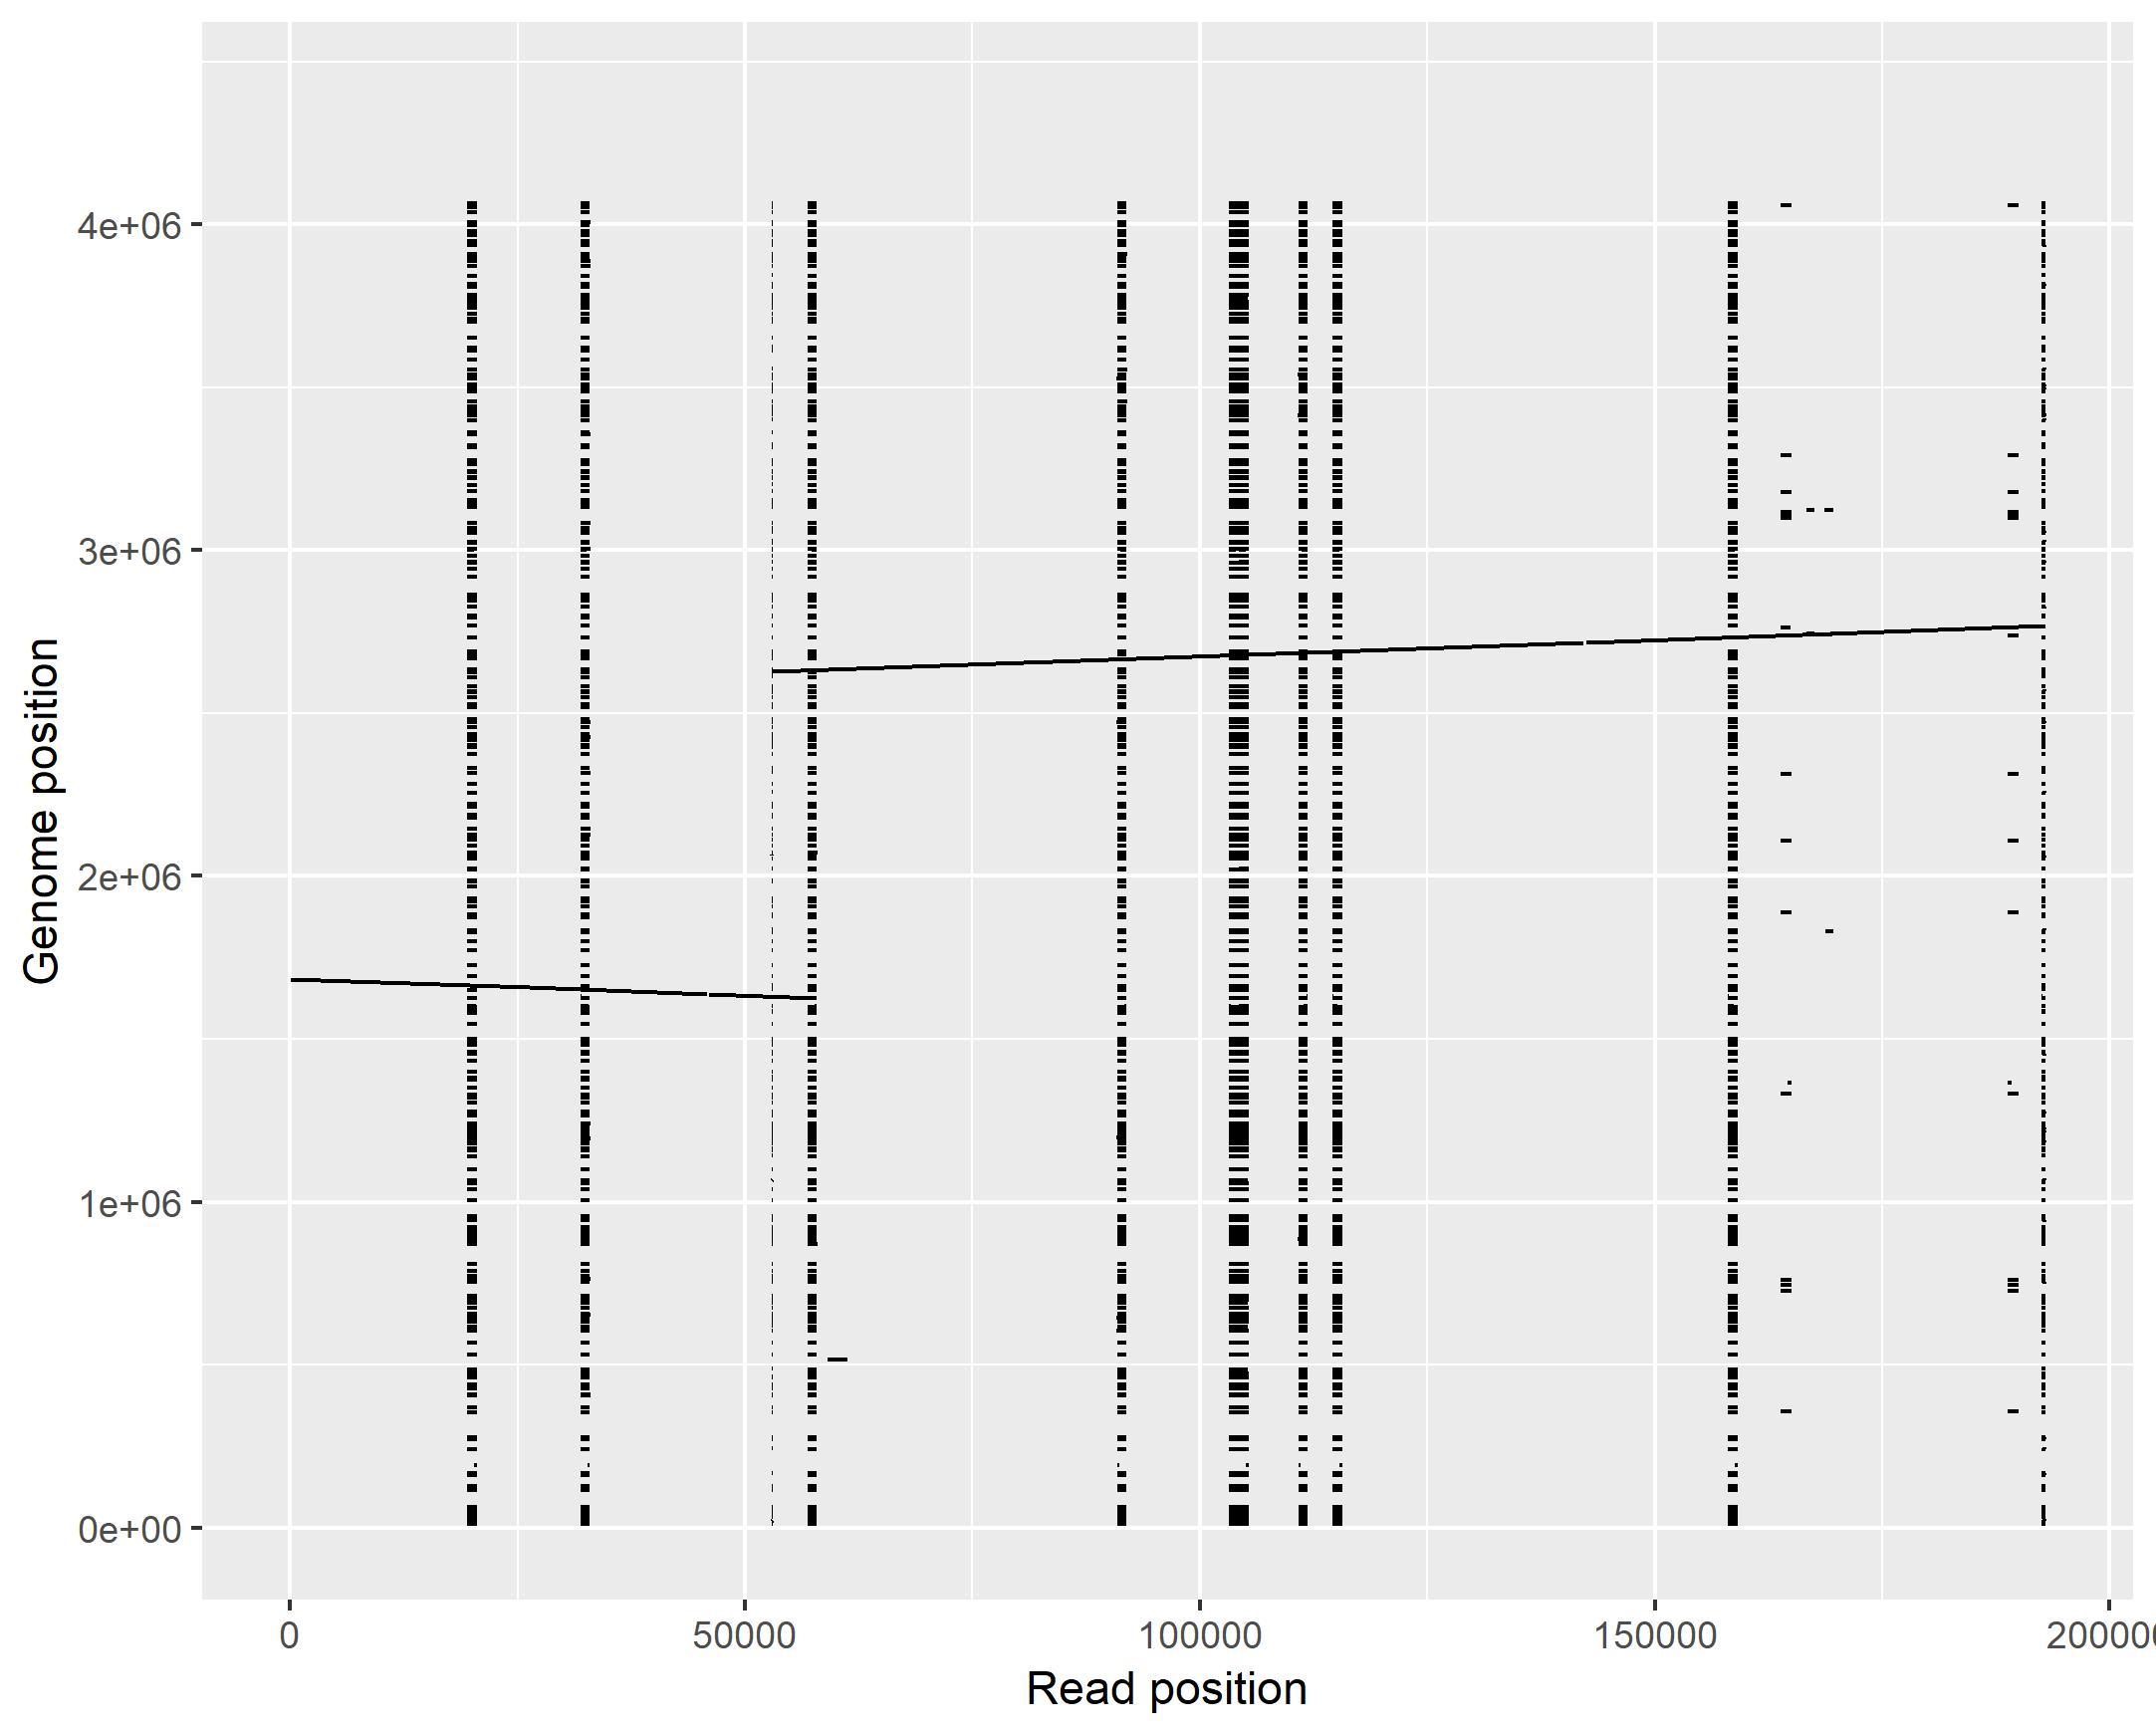
\includegraphics[width=\textwidth{}]{Chapter_2/Blast_results_381179.jpeg}
\caption{A read which had no evidence of being a chimera but also appears to be a genome rearangement. The pre junction DNA from 0-53kb on the read (x axis) is in the inverse orientation to the genome (Y axis) as it matches in a negative orientation (appearing as a negatively sloped line)- starting at 1.63Mb and ending at 1.62Mb in the consensus sequence. The DNA after the junction,however, is positively orientated with the consensus sequence (appearing as a positively sloped line) - the read sequence from 53kb-200kb matches from 2.62Mb to 2.76Mb on the consensus sequence. }
\label{fig:Inv_are_possible}
\end{figure}

\begin{figure}[h!]
\centering
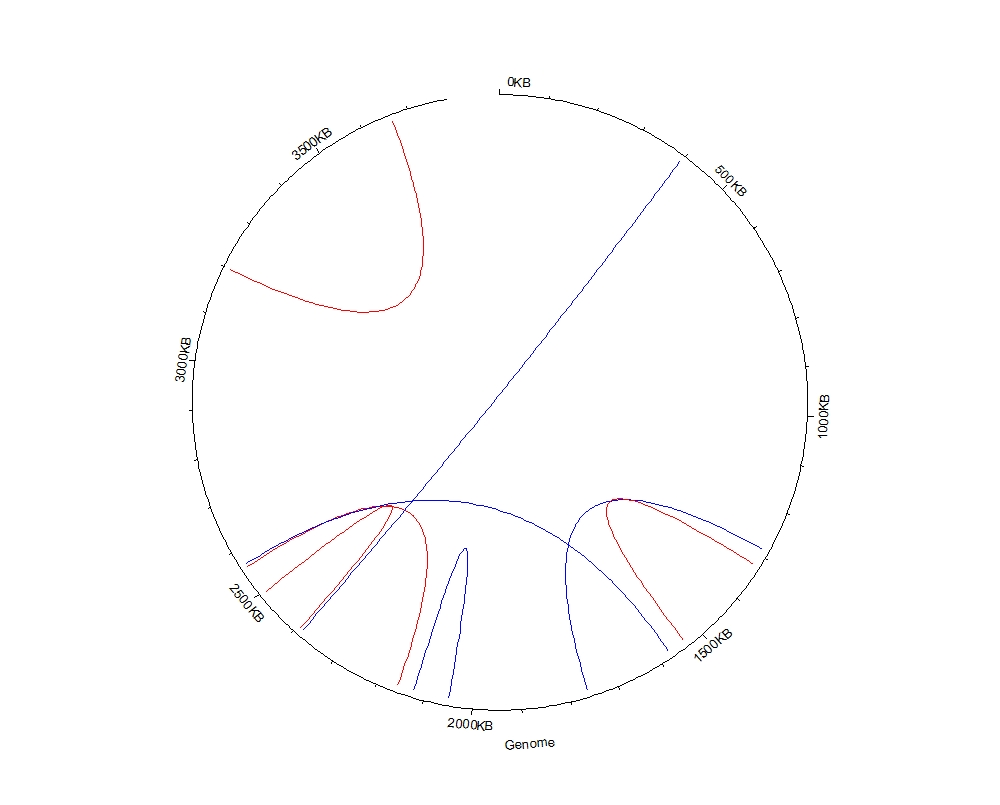
\includegraphics[width=\textwidth{}]{Chapter_2/Rplot05.jpeg}
\caption{A circos plot showing the 8 reads with no evidence of being a chimera. Blue lines indicate reads which are duplications or deletions and red lines indciate reads which are rearangements. }
\label{fig:Final_baskey}
\end{figure}
%Probs a table here with the results. Real read names,locations etc.

%A paragraph explaining some trends of this data
Using this method it could be demonstrated that putative SVs in single reads that were not present in the consensus sequence could be isolated. However in this sample, there were only 8 such reads. Whilst it appears that there was a slight bias of reads towards the terminus, that wasn't repeated in the following analysis of UK76. What this data does demonstrate,however, is that the BP genome is highly plastic and this can be observed in as little as two passages using Nnopore reads.

\subsubsection{UK76 contains many weird junctions}

Having established that structural variations could be detected in single Nanopore reads in the UK54 dataset, it was important to establish this phenomenon in another sequence dataset.

The strain UK76 presented one of the largest CNVs at >300kb (with a tandem length of >600kb) and had a predicted Copy number of this locus as 1.3. This strain was sequenced as part of a generic investigation into CNVs in B.pertussis. Unsurprisingly, no reads were found to span the whole tandem array.

Undertaking the same analysis on this sample provided insight into CNV formation in B.pertussis. Of the ~400k reads generated, 136 reads were found to contain DNA sequences that were proximal on the read but distant on the consensus sequence of which 95 were found to have junction sequences in repeat elements. Of these 95, 67 had no adapter sequence or homology gaps at the junction -remarkably higher than 8 reads passing the same tests in the UK54 sample.

It was found that UK76 had multiple different CNV junctions present in the sample (Figure \ref{fig:UK76_baskey_1)}. Whilst previous experiments demonstrated that heterogeneity of copy number was possible, these results indicated that heterogeneity of the sequence composition of CNVs was possible within a single sample. 


\begin{figure}[h!]
\centering
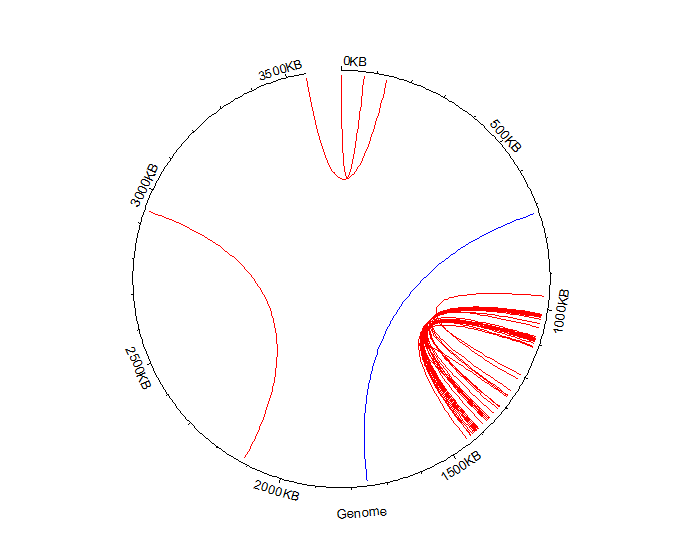
\includegraphics[width=\textwidth{}]{Chapter_2/Rplot136.png}
\caption{A circos plot showing the 67 reads with no evidence of being a chimera in UK76. Blue lines indicate reads which are duplications or deletions and red lines indciate reads which are rearangements. Many reads with slight variation in junctions were found between 0.9Mb and 1.5Mb.}
\label{fig:UK76_baskey_1}
\end{figure}

Further analysis of these results showed that 20 reads had a break point of 1.315Mb to 1.709Mb. This matched the predicted CNV in Chapter 1, an estiamte based on illumina data of the same sample. There were many reads which had subtle variations of this, however, with breakpoints differing by only a few 1000 bases. These appeared also to be true. There were drastically different breakpoints too which I explored.

\begin{figure}[h!]
\centering
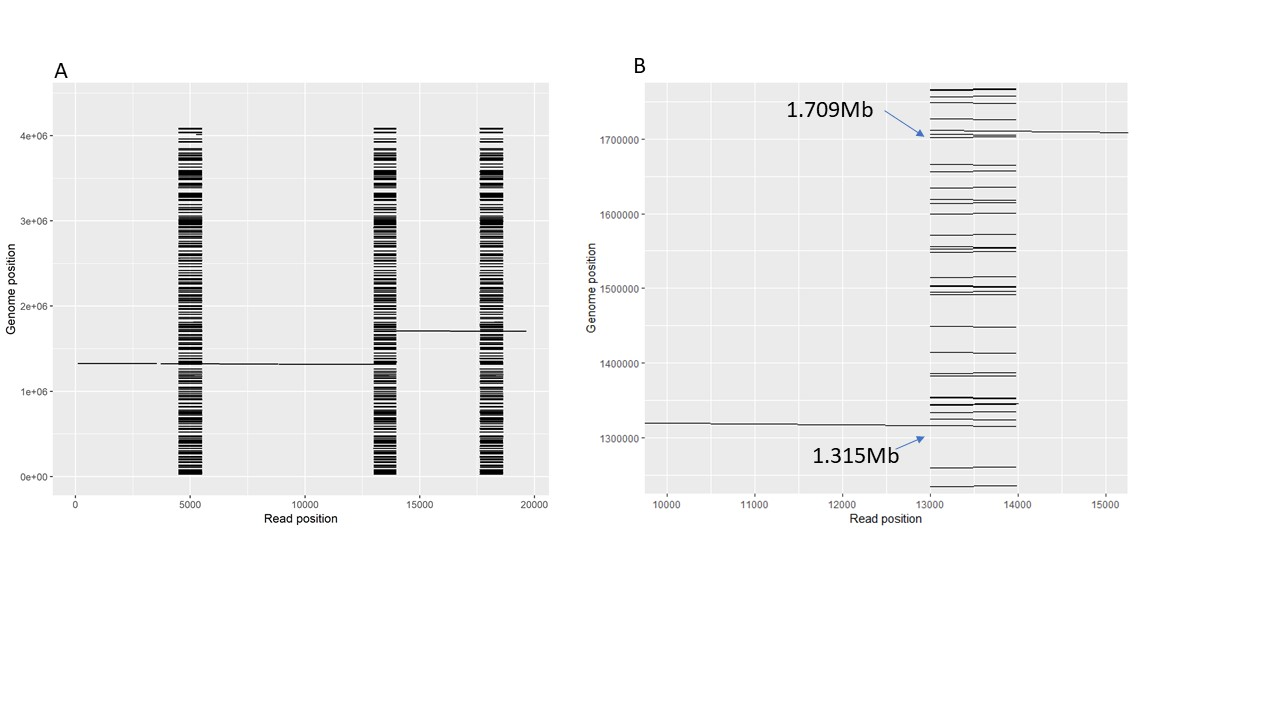
\includegraphics[width=\textwidth{}]{Chapter_2/Popular breakpoint.jpg}
\caption{An alignment between a read with the most frequent breakpoint (A). The junction is enlarged in (B). The breakpoint was 1.315Mb-1.709Mb}
\label{fig:UK76_most_popular}
\end{figure}

The second most popular configuration was  1.385Mb-1.655Mb where at least 6 reads had the breakpoint, again with subtle variations.


\begin{figure}[h!]
\centering
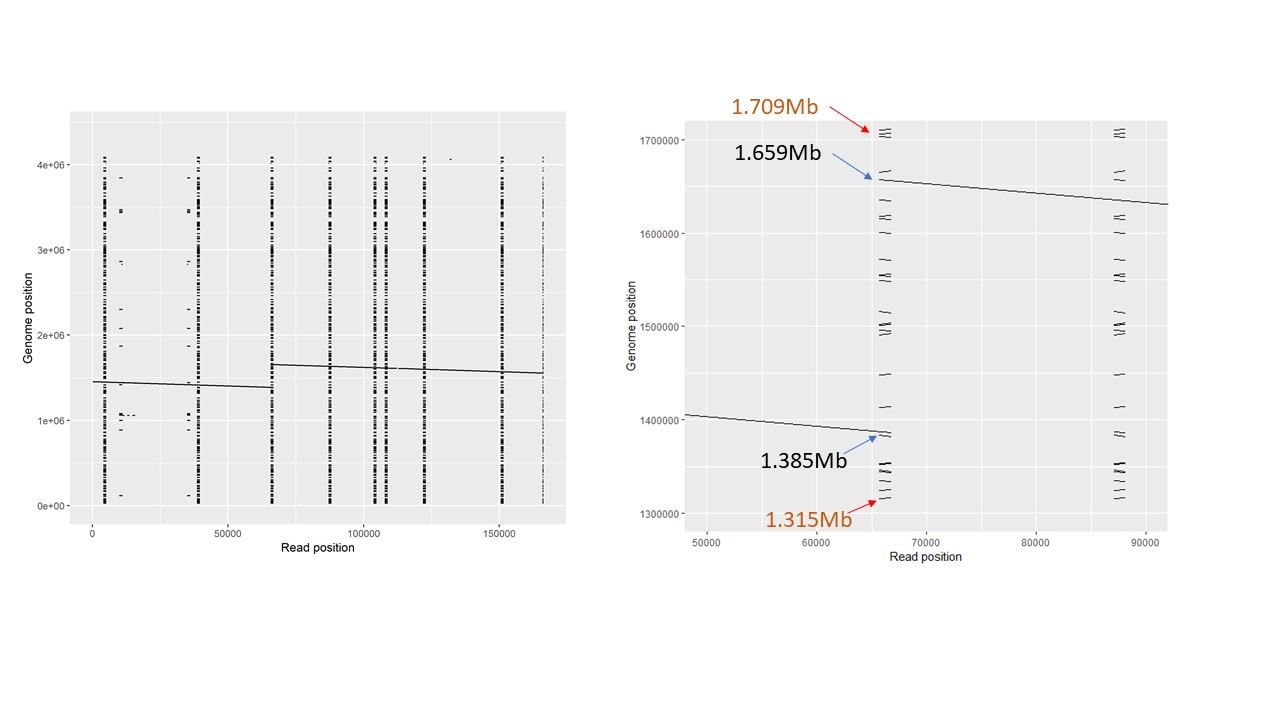
\includegraphics[width=\textwidth{}]{Chapter_2/second most pop.jpg}
\caption{An alignment between a read with an alternative breakpoint (A). The junction is enlarged in (B). The breakpoint was 1.385Mb-1.655Mb. In red is the breakpoints found in Figure \ref{fig:UK76_most_popular})}
\label{fig:UK76_second_popular}
\end{figure}

There was a small amount of reads that appeared to have their own unique junctions. Whilst it was unfeasible to manually check each break point, every new break point configuration that was manually analysed indicated that the basketball analysis was true. There were at least 4 breakpoints present in this sample: 2 popular (Figures \ref{fig:UK76_most_popular} and \ref{fig:UK76_second_popular}) and 2 rare/unique ((Figures \ref{fig:UK76_third} and\ref{fig:UK76_fourth}).

\begin{figure}[h!]
\centering
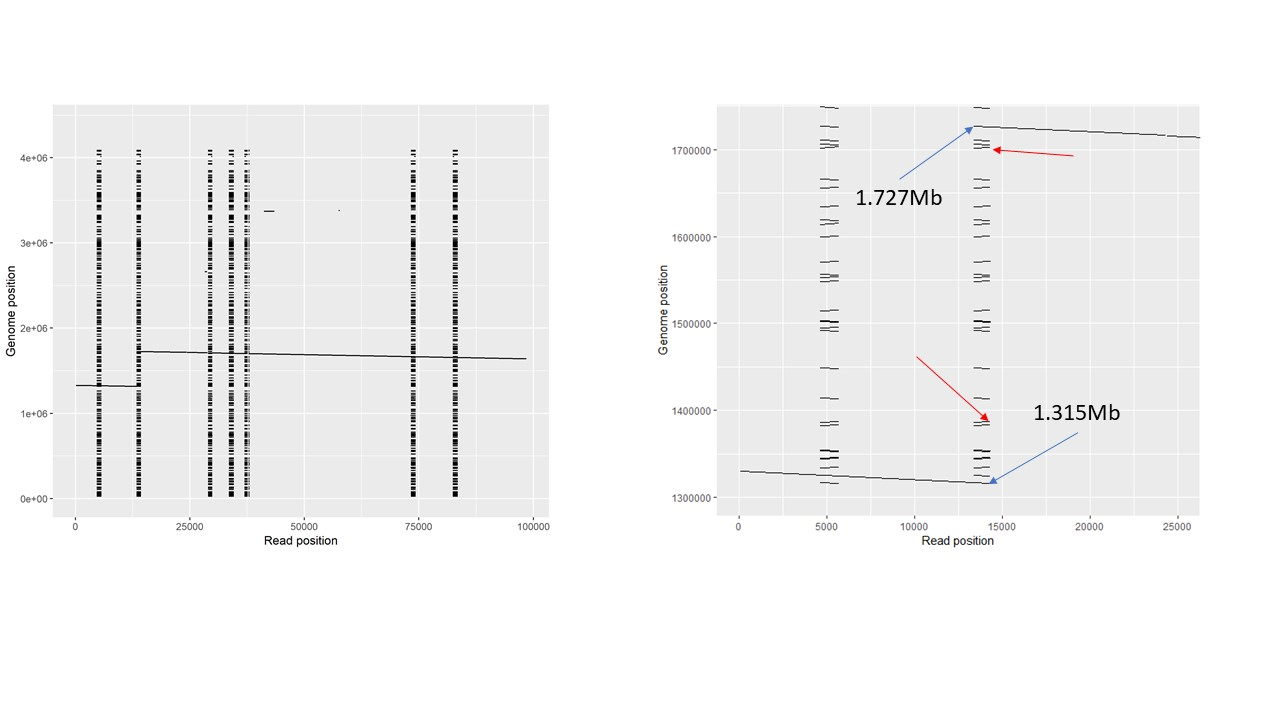
\includegraphics[width=\textwidth{}]{Chapter_2/third unique.jpg}
\caption{An alignment between a read with an alternative breakpoint (A). The junction is enlarged in (B). The breakpoint was 1.315Mb-1.172Mb. In red is the breakpoints found in previous analyses but not in this read (\ref{fig:UK76_most_popular} \&Figure \ref{fig:UK76_second_popular}}
\label{fig:UK76_third}
\end{figure}


\begin{figure}[h!]
\centering
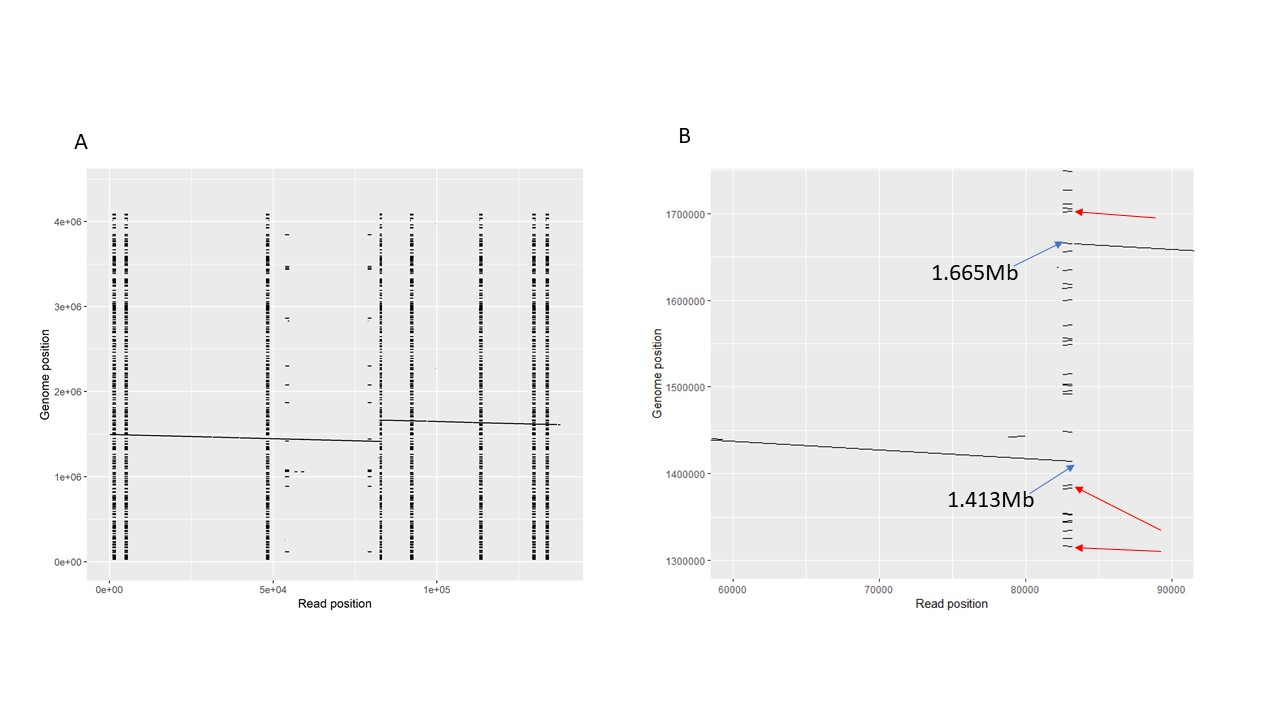
\includegraphics[width=\textwidth{}]{Chapter_2/junction 4.jpg}
\caption{An alignment between a read with an alternative breakpoint (A). The junction is enlarged in (B). The breakpoint was 1.413Mb-1.665Mb. In red is the breakpoints found in previous analyses but not in this read (\ref{fig:UK76_most_popular},Figure \ref{fig:UK76_second_popular} and Figure \ref{fig:UK76_fourth}}
\label{fig:UK76_fourth}
\end{figure}

This analysis of UK76 therefore was a valuable experience. It was clear that in this sample a high amount of genome plasticity had been observed. I had,however, hypothesised that there would be frequent de-novo SVs all around the genome,fairly consistently and in the UK76 sample this was not the case. Like other BP isolates from the 2012 epidemic, it was unclear if these samples had been isolated from a single colony on a plate or the observed diversity was generated in-vivo and had been captured by taking a sweep of the plate. It cannot therefore be concluded whether this vast diversity of breakpoint occurred during in-vitro passage or in-vivo.

As this methodology was resource intensive and not all steps could be automated at the time of writing, I sought to understand how well developed and highly efficient assembly algorithms handled such divergent and often unique reads.


\subsection{Mining assembly graphs for data to back this up}
%Further to this, We could also show that assemblers were overlooking this data/were not sure what to do with it.

It has been previously reported that long read assemblers have failed to assemble BP genomes predicted to contain long tandem duplications. Assembly is not a single stage process,however, and there exists many intermediate steps that generate data. I investigated a number of intermediary genome assembly graphs in the assembly process of Unicycler to investigate how this data corroborates my basketball analysis and to generally explore the assembly process for any potential utility.

As Ring et al noted in their assemblies, use of Nanopore reads with Illumina reads in a hybrid assembly resulted in a single contigs but with the probable CNVs collapsed. Conversely, assembling just long read data also gives a bad assembly although with different flaws. The results of the Ring et al assemblies were were replicated here, but only in unicycler and without any short read data.


%{Explanation of de- bruijn graphs and how the intermediate steps can be interpreted for our use}


The genome UK48 had a predicted duplication size of X and it had been sequenced with ultra-long Nanopore sequencing in an attempt to resolve the duplication. Like other samples,however, it was not possible to resolve the CNV.

Assembling long read data for UK48 with unicycler gave a fragmented assembly of 12 contigs and a total assembly size of 4.4Mb- 300kb longer than would be expected if the duplication was not resolved (Figure \ref{fig:Graph_blast_1}). Blasting the putative duplicated region, in addition to considerable flanks either side, against this graph revealed that the duplication had approximately 130\% coverage in the assembly and was spread over multiple contigs- one of which contained 40\% of the duplication and was noted in the genome assembly graph as having a copy number of 1.52. It therefore appeared that the duplication was partly resolved, although it is unclear which parts had been collapsed to a single copy

Using the same 'blast-to-graph' methodology it was clear that one contig was a junction sequence between the tandem duplication - direct evidence a duplication is present in this sequence. The ability to resolve junction sequences from sequence data is a clear advantage of long read Nanopore data.

\begin{figure}[h!]
\centering
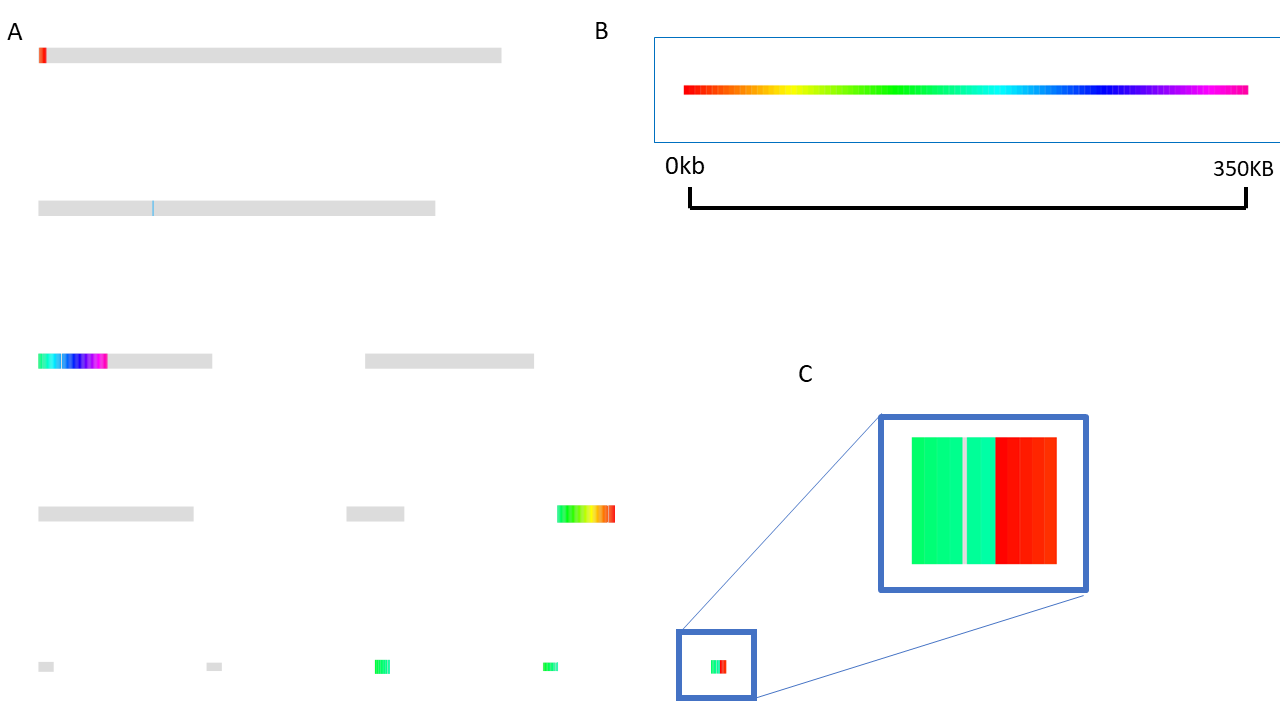
\includegraphics[width=\textwidth{}]{Chapter_1/blast graph 2.png}
\caption{UK48 was assembled to 12 contigs (A) and the putative duplication sequence, with flanking regions, was searched against the assembly(B). The rainbow colour spectrum (red,orange,yellow,green,blue,indigo,violet) is used to show matching sequences in the subject(the assembly) to the query (the duplication). Panel C shows a closer examnation of a contig: green sequences are adjacent to red sequneces, despite these sequences being seperated by ~160kb on the query sequence (B).The contig therefore appears to be a junction sequence.}
\label{fig:Graph_blast_1}
\end{figure}


In order to further understand the assembly process and data which gave rise to such an assembly, the UK48 string graph was examined. In this graph, the >500k reads have been reduced to a less redundant set, although with much redundancy still present. The duplicated region was shown as a complex structure with reads that were clearly junctions and a `bubble' that contained the duplicated sequence. Examining this graph revealed the complexities of long read assembly in Bordetella pertussis. Such junction sequences can be used to, in combination with other sources of evidence, automate the construction of hypothesised duplications in the future. This could provide a genome which is of a quality intermediate between fully resolved and partially resolved. This task, however, was outside of the scope of the current work and would struggle to resolve very complex CNVs such as those outlined in Figure \ref{fig:B199}).

Intermediate assembly graphs were useful in their own right as they supported my previous work on the diversity of junction sequences in UK76.  In the UK76 basketball plot it could be observed that there were many reads indicating a duplication or deletion but that had a variety of start and end points- these results could be observed in the genome assembly graphs. By conducting a BLAST search for the duplicated region (with single copy flanks) we could identify many sequences that were SV junctions. Further investigation into these reads corroborated the work from the basketball plot: there were reads showing different breakpoints thus indicating multiple duplication events co-occurring within the population. Unicycler was discarding these reads, likely because of their divergent gene content. We could therefore show in two independent ways, analysing the same dataset, this novel feature of the UK76 sample. 



\begin{figure}[h!]
\centering
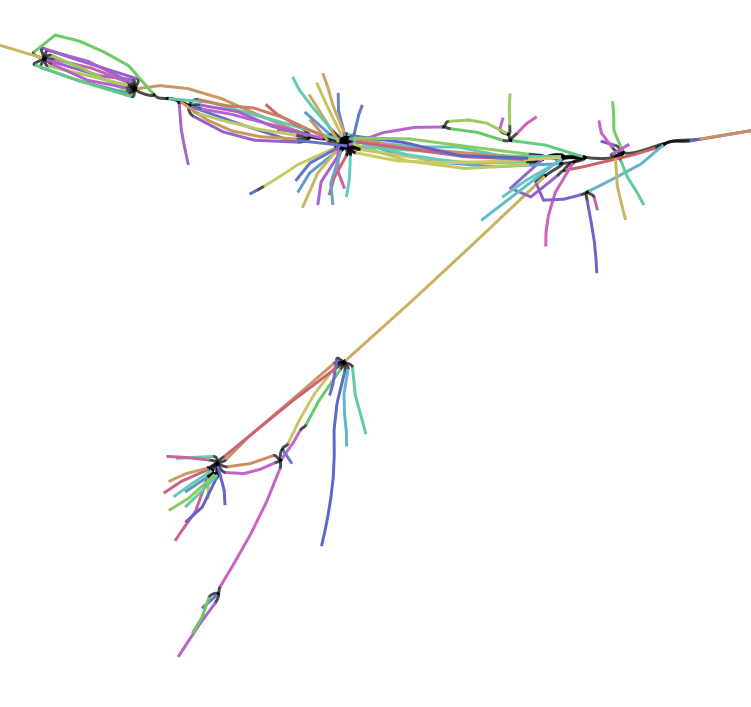
\includegraphics[width=\textwidth{}]{Chapter_1/graph.png}
\caption{ A subset of the UK76 assembly graph, midway through the assembly. Randomly coloured.}
\label{fig:MDR_Man_PC3}
\end{figure}

\begin{figure}[h!]
\centering
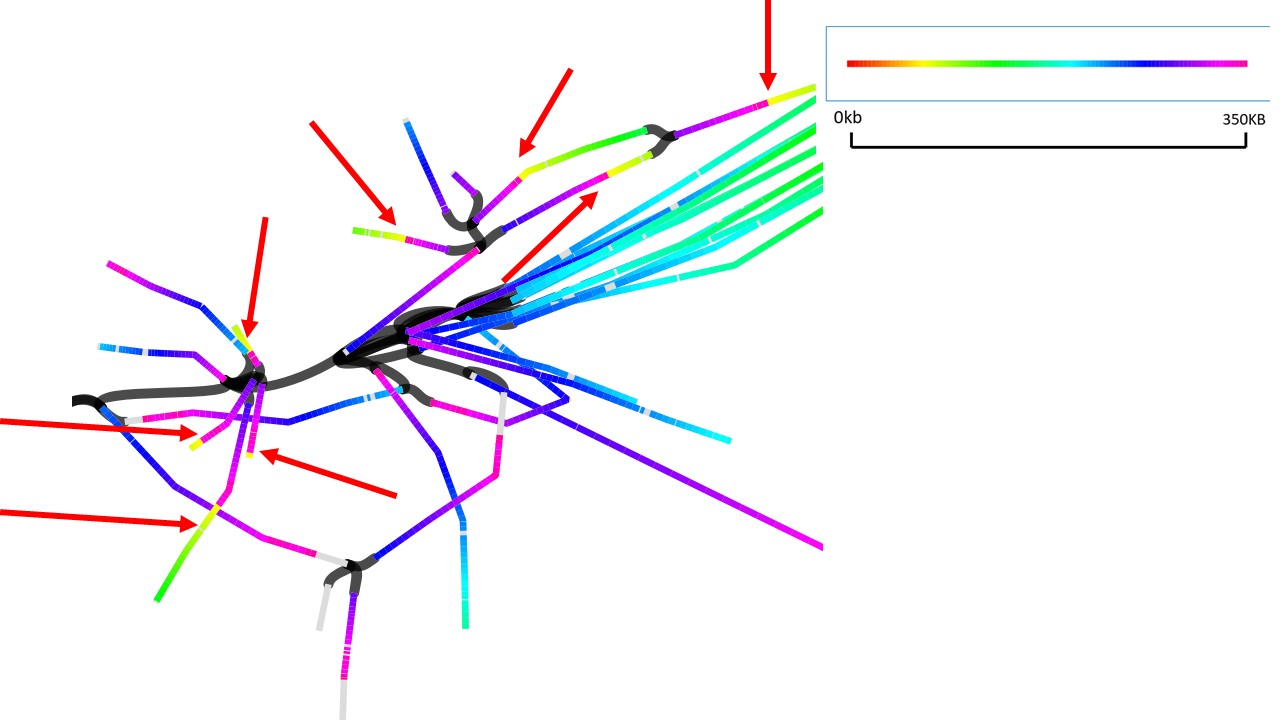
\includegraphics[width=\textwidth{}]{Chapter_2/labelled mid-assembly ting.jpg}
\caption{An early stage of the assembly was examined further. Nodes with juxtaposed colours (yellow to blue) rather than continuous colour spectrum s(blue-purple-green-yellow) were observed and indicated with large red arrows. Such nodes represent junction sequences.}
\label{fig:MDR_Man_PC3}
\end{figure}



\section{Discussion}
 
\subsection{Copy number estimates using short read data predicts mixed populations}


In the work outlined here, I expanded on the data generated in Chapter 1 to reveal the likely existence of mixed populations of cells in Illumina sequencing samples.I then  extended on this by using Nanopore sequencing to capture either whole tandem arrays of CNVs or junctions between CNV copies in single Nanopore reads.


%I found there were intermediate copy number estimates
The cohort of >2700 BP isolates from Chapter 1 was reanalysed to find that many of the copy number estimates were not integers. This was in addition to the copy number discrepancies described in Chapter 1 in the manually resolved dataset. I hypothesised that this is because cells in the population have different copy numbers of the locus and when an average is taken (as is the case for read depth based estimates), the value is intermediate between the true copy numbers.

%This was because
Non-integer estimates could be, at least partly, due to inaccuracies of CNVnator estimating the copy number via read depth. If CNVnator was estimating copy numbers inaccurately there is no evidence to suggest it wouldnt do so randomly, following a normal distribution. The observed pattern of intermediate copy number estimates in both the full cohort dataset and the cohort of isolates with resolved duplications ,however, did not show such a distribution (Figure \ref{fig:Full_data_discrep} and\ref{fig:CDC_discrep}) . Both distributions of copy number estimates in the two datasets were skewed towards lower copy numbers rather than an even normal distribution around integers. For example, in the manually resolved duplication dataset, of the 25 CNVs that were approximately copy number 2: 5 were exactly copy number 2; only one was considerably abouve 2 (copy number 2.3) and 12 being considerably lower (<1.9). If these estimates were not explained by a normal distribution of inaccurately estimates centered on integers, it also could be that CNVnator systematically underestimates copy numbers. This theory, however, has no evidence in the literature. The hypothesis that such estimates were produced by a biological process was therefore strong.

%This led to..
As the short read CNV predictions indicated mixed populations, it was therefore investigated whether long reads could capture whole tandem arrays of CNV loci and demonstrate the mixed populations of cells.

%https://www-pnas-org.ezproxy1.bath.ac.uk/content/pnas/78/5/3113.full.pdf
%CNVs are unstable

\subsection{Nanopore sequencing confirms mixed populations}

\subsubsection{Ultra long Nanopore reads can resolve tandem arrays}
%RawResult:I found a tractable CNV

The CNV estimates generated in Chapter 1 were used to screen for a CNV that was genetically tractable. In this instance, this also happened to highlight the CNV with the highest copy number in the large cohort dataset. The UK54 strain had a CNV that was 16kb long in its single configuration, its full tandem configuration was predicted to be 64kb- a tractable size to be sequenced on the Oxford Nanopore Minion. Regular protocols produce reads with an N50 of ~5-10kb which is not adequate to sequence this CNV in its tandem configuration. As the Nanopore platform can theoretically sequence unlimited length reads, given careful DNA and library preparation, much longer reads can be generated. To this effect, the ultra-long read protocol was followed.

%RawResultWe sequenced this CNV successfully and saw...
Sequencing UK54 using ultra-long reads demonstrated that a mixture of copy numbers could be isolated. This was a successful experiment in two ways: resolving the duplication and demonstrating that there was a mixed population.
%This was because: 

%Need to put in the text the stats behind UK76 and UK54 not mixed. These were actually much better runs.
Whilst still in its infancy, ultra-long read generation on the Nanopore has been shown to be effective previously. High N50's, low amount of short read data etc has been demonstrated. Whilst this sequencing run of UK54 had an N50 of x and had many short reads, there were also many long reads- a `wider' distribution of read lengths was generated. The subsequently sequenced UK76 and the 3 UK54 clones had much better sequencing statistics, with N50's of X and Y. In the future if this could be improved, it is likely that it is possible to resolve larger duplications. In particular, if less DNA was highly fragmented to below 5kb , more of the sequencing capacity of the minion could be used for long reads. 
a

%Broad analysis:
Because of the distribution of read lengths within a sequencing sample(Figure \ref{fig:Read_counts}), it is much less likely to isolate a read with a higher copy number. There was,therefore, no attempt here to use these single reads to quantify the average copy number of the sample as each copy number, from 1 to 5, would have a different minimum read length needed to observe it and therefore a different chance of being observed, given the spectrum of read lengths generated. It is more reliable to use the read depth as this is derived purely from how many reads covered that position with no stipulation of their length.
 


%This led to...
%We were not sure if our samples were clonally derived, therefore isolated single colonies
It could not be confirmed if the original stock of UK54 had been clonally derived. Public Health England guidance suggests that multiple single colonies from a plate can be used to seed liquid culture. This is a good way to represent the diversity of bacteria from the sample and will assist in accurate phenotyping. For example, there may be a mixture of antibiotic resistant and sensitive isolates on the diagnostic plate and picking a single colony would inaccurately describe the antibiotic resistance profile of the sample. This means that many BP samples contained on the SRA may infact not be clonally derived, despite the assumption that the opposite is true.

In order to definitively ascertain that CNVs were highly plastic in BP, it was necessary to repeat the experiment with clonally derived samples.



\subsubsection{Mixed populations from clonally derived isolates}

%RawResult: Mixed populations persisted
%Single colonies gave a variety of copy numbers. 
%This was because...

Eight clones from the UK54 stock were isolated and their copy number established using qPCR. Similar to read depth, this experiment assays the average copy number for the whole population. using qPCR in this way was therefore used to screen for copy number differences and to select which clones to sequence. 

The results from sequencing clone 4 clearly indicated that mixed copy numbers could still be recovered as reads with both 5 and 2 copies were found. This therefore means that culturing UK54 from both single colonies and the original stock produced the same result. It could therefore be established that copy number changes were being generated rapidly during limited in-vitro passage. 

%Whole CNV loci were only isolated in UK54 clone 4 and not 8 because clone 4 had a tractable average copy number of 4.32 whilst clone 8 was not tractable at 51 copies. 


%This does not exclude the possibility that the observed genome plasticity of the original mixed sample of UK54  also happened in-vivo. 

It is possible that UK54 clone 4 had fewer complete reads of the locus (3) compared to the original UK54 population (9), because it was a culture that had been sub-cultured fewer times and therefore less genetic diversity was observed. The UK54 clone 4 did  however, have two reads isolated in with 5 copies of the locus and 1 read with 2 copies of the locus-enough to prove that the copy number was plastic during brief passage. 
%Broad analysis/lit: UK54 CNV instability supports intermediate copy number predictions. 
%this is a really big point. Probably the biggest of the thesis.

%This is really interesting because if copy number change is so rapid, we would never expect to see CNVs in the global population.
Finding that brief in-vitro passage can lead to intermediate copy numbers supports that the `inaccuracies' of copy number estimates from Illumina data generated in chapter 1 were due to populations of mixed genotypes being sequenced. This evidence indicates that entering clinical isolates into in-vitro passage leads to mixed populations of cells to be generated. This is highly interesting and one of the key results of the thesis.
%in-vitro instability of CNVs is a logical counterpart to the thoery that CNVs are formed in-vivo and under a selective pressure
%THree points must be combined here:
	%We observed in-vitro plasticity to the point of a low sensitivity method picked up plasticity
    %Whilst CNV occur frequently, in order for them to get to fixation and be noticed on a global scale they must be reach fixation within their small sample.
    %Global cohort showed lots of CNVs
%As later on we demonstrate that we can detect mutants at low frequency but in clone 4 1/3 of the data was copy number 2.
%Need some help here
%As capturing whole tandem arrays of CNVs relies on long reads being in exactly the right place, it is a low sensitivity method. It is therefore even more noteworthy that copy number changes were observed during in-vitro passage.As in-vitro plasticity was observed leading multi-copy regions to quickly diversiy, despite this method having a low sensitivity
%This data supports the hypothesis generated in Chapter 1, that CNVs are formed by selective forces in-vivo. 


%This data shows that copy number changes from a multi-copy locus to


%If CNVs are so unstable in-vitro, and it is known that
%In-vitro instability of CNVs is a logical counterpart to may not be If CNVs were so unstable during in-vitro passage this suggests that continual culture in-vitro would lead to a return to single copy. 

%This is a vital next step to the work presented here. 


%
%The observed distribution of copy numbers in these two analyses fits closely with the known dynamics of CNVs in bacteria. Once a region has become a duplication, it is highly unstable and is highly likely to return back to single copy. This is because duplicated stretches of DNA are able to recombine again to cause a deletion.

%Clone 8 had an uber high copy number. Tandem arrays are highly unstable. This likley caused it. How often is this occuring though and how lucky were we to find this? FACS?

%This led to


\subsubsection{`Extreme' gene amplifications}
One of the most surprising results generated here was the isolation of a clone with a copy number of 51. Whilst such an outlier was at first approached with skepticism, read depth coverage on the Nanopore platform agreed with the qPCR results. 
 
It is widely known that tandem arrays are highly unstable and that instability increases with copy number. Such knowledge comes from experimental systems which are manipulated with extreme in-vitro selection pressures such as antibiotics. Whilst genetic variation is constantly being produced, it is filtered by selection. Therefore if 1000's of UK54 clones had been studied, we might expect to see some `extreme' copy numbers, yet in the present study only 8 clones were studied. This brings up the question as to why such an extreme copy number was observed here with limited sampling. It is unlikely that just by chance alone that such a clone had been selected and as such it is more likely that CNV instability is so great that there are many clones in the population with extreme copy number, greatly increasing the odds of isolating this type of clone.

`Extreme' gene amplifications have been studied in bacteria for decades, although mostly in non-pathogenic experimental systems. A recent landmark study by Nicoloff et al was able to demonstrate clinical isolates of several species contained copy number variable repeats and the isolates were able to rapidly amplify their native antibiotic resistance cassettes ,in some cases upto 100 copies, in response to antibiotic challenge invitro. Whilst these isolates were clincally derived, they underwent extreme amplifications in response to extreme selection pressures. The most important parallels between the Nicoloff et al study and the work presented here is that both studies are observing amplification of genes using systems native to the isolates, rather than relying on an experimental system. This highlights the need to understand more about the UK54 population and why such a high copy number clone had been isolated. 

%Long-read Nanopore sequencing of two clones of UK54 led to the remarkable observation of a CNV with average copy number of 51. It is a well-documented phenomenon that multiple copies of a locus in tandem greatly increases the instability of the locus. In experimental systems, copy numbers of up to 100 have been generated 42 and in clinically derived isolates the copy numbers of antimicrobial resistance genes can change rapidly, increasing up to 70 copies in response to antibiotics 46. Whilst the function of the genes in the UK54 CNVs are unclear it is possible that they provide a fitness benefit to the strain under certain conditions. What is strange is to have isolated such a high copy number without trying.

\subsection{Technical hurdles to studying SVs in single nanopore reads}

It was observed that the copy number of CNVs was plastic during brief in-vitro passage. The previous analysis, however, only studied the locus that was expected to change. I therefore investigated if similar events were happening genome-wide during passage.


To search for genome-wide SVs it was necessary to compare each read to the consensus sequence. This was a technical challenge and required two optimisation steps that were outlined in the Results: Ensuring reliable BLAST results were generated and removing chimeric reads.


\subsubsection{Analysing BLAST results used steps that may have reduced the true positives}
When a section of the read matches two or more sections of the consensus sequences it is highly challenging to identify which is the most appropriate match and if this match is expected. This was overcome in two ways. Firstly, the consensus sequence was depleted of any 1kb stretch of DNA that had a homology match in at least 50\% of its length to any other region of the genome. This highly permissive threshold meant almost 1Mb of DNA was removed from consensus genomes. This succesfully removed most ambiguous sequences. Where small stretches of read DNA matched to multiple places in the consensus genome, the section with the highest BLAST score was chosen. Combining these two methods of BLAST result analysis resulted in a high confidence dataset that truly identified reads which contained juxtaposed DNA sequences.

Such an extensive depletion of repeat sequences in BP may have reduced the amount of SVs that were found. This is because whilst there are approximately 270 repeat sequences per genome, most of which were 1kb, there was more than 1Mb removed. This was approximately 4x more than is to be expected (~270kb). Whilst this produced high quality data, there is likely more reads in these datasets that contain SVs. However it could be demonstrated that the method presented here generated a high confidence dataset and so this trade-off appeared worthwhile.


\subsubsection{Identifying probable chimeric reads}

The second crucial step of this analysis was to delineate real SVs from chimeric reads. Whilst real SVs have a number of recognisable hallmarks, many are of these are  shared with chimeras. The main distinguishing feature of chimeras and true SVs is the presence of an adapter sequence partway through the chimeric read which is   recognisable either directly or indirectly. This process is frustrated by the raw error rate of the Nanopore platform chemistry used here, which was 10-20\%.  I therefore investigated the dynamics of adapter searches on simulated DNA.

By undertaking adapter homology searches on simulated data, it could be demonstrated that adapter sequences could be expected to match random DNA sequences at 50\% homology. For the chimera-sensitive application here this meant that in order to eliminate 99\% of chimeras, 34\% of non-chimeric reads would be be identified as chimeras in at least once location on the read. This was an unacceptable level of false positives  given that the application proposed here needed was very sensitive to chimeric reads. An alternative methodology was therefore investigated. This is based on the fact taht

A limitation of this simulation was that many real features of Nanopore biases were not simulated. The only factor considered was the GC content, however, errors in Nanopore data are not random, but instead have specific biases. It is likely that using a complex model to simulate Nanopore data would give different results, although accurately simulated data is unlikely to drastically effect the results. 


%ELECTRONIC SIGNAL

An avenue of future research into the identification of chimeras is to investigate other identifiers of chimeric reads. During Nanopore sequecning, the final DNA sequence of each read has been interpreted from the raw electronic signal the DNA molecule made as it passed through a nanopore. At this signal level, there may be evidence of chimeras that was misinterpreted or missed. This appears to be true for both in-sillico chimeras (two reads passing through the pore in quick succession) and true chimeras (Two DNA molecules attached by adapter sequences).

%R10 less error,
%https://www.biorxiv.org/content/10.1101/645903v3.full.pdf
%https://nanoporetech.com/sites/default/files/s3/posters/pdf/R10%20Evaluation_Shanghai_NTT_2019.pdf

Repeatign the work proposed here with new Nanopore chemistries, which promise improved errors rates, may make chimera detection more reliable. Preliminary research of the  R10 sequencing chemistry on the Oxford Nanopore sequencing platform shows  that is is possible to reduce the raw error rate of reads to 5-10\%. This would greatly enhance the ability to detect chimeric reads, although direct comparisons of chimera rates for the R9 and R10 chemistry has not been performed as of yet.


\subsubsection{Removing adapters via homology search is effective}
Given that there was a lack of pre-existing tools and/or data to identify chimeric reads with very high sensitivity and specificity, alternative methods were undertaken.
%Porechop is used alot. Our data shows that this would be unacceptable

%. Reference guided adapter exclusion was the best here.,
 Adapter sequence searches were combined with read-consensus homology searches to indicate if a read is likely to be a chimera. The results showed that  gaps in alignment between the read and the consensus sequence were highly correlated with adapter sequences present. In the cases where adapter sequences were not found but a gap had occurred, it can be assumed, due to the close relationships between gaps and adapters, that this `foreign' DNA is a highly degraded adapter sequence. Therefore any read which contained an adapter or gap directly adjacent to the repeat was excluded. This was a highly effective strategy which produced reads which had no evidence of being chimeric.
 
Due to the results of the simulation study (Figure \ref{fig:Histo_homo} and Table \ref{tab:Homo_example}), it was decided not to just simply rely on string-matching tools such as Porechop. Porechop is one of the most popular read trimming tools which removes adapters from the start/end of reads and splits reads or deletes them if adapters are found in the middle. 

%Shunt this to discussion
It is technically possible to rely on Porechop with a low adapter homology threshold to split chimeras- even though this may produce many false positives. The resulting highly fragmented set of reads would likely still contain the right information ( e,g reads containing DNA from two different parts of the genome adjacent on the read). There are many disadvantages to this strategy however and it was not pursued for the following reasons. The primary concern was that there would be less `anchoring' DNA on either side of the junction leading to a harder analysis for some reads and given that porechop may split at least  34\% of the reads .  A second reason was that as each read in the raw data was split into an individual file and porechop would make extra files, the running of the method presented here would become more technically challenging.

%Our data highlights that if it is absolutely imperative that chimeras are caught, then it is very important to not just solely rely on porechop
 
The research conducted in this chapter on adapter sequences and homology gaps in read-consensus alignments indicates that if it is imperative to find chimeric sequences with minimal false positives then the method presented here, reference guided adapter exclusion, performs well.
 
\subsubsection{Computational inefficiency results in inconclusive data}

Using BLAST to find reads with juxtaposed DNA sequences is resource intensive and therefore only two samples were investigated. The most compute intensive task is the  BLAST search itself which compares each read to the consensus sequence. This step takes roughly 24 hours to run whilst the rest of the analysis can be carried out in approximately 6 hours. There is therefore scope to drastically improve the efficiency of this method.

One method to speed up this process would be to rely on pre-existing mapping pipelines which are well designed for the task of homology searching. Most of these tools  will mark reads which do not fully align to the consensus sequence by either noting a `not primary alignment' or `supplementary alignment' value in the FLAG field of the SAM file format. Any read that doesn't wholly and uniquely map to the reference sequence would be noted with these warnings.  Whilst all the SVs noted here would be highlighted in this way, an additional source of supplementary alignments from a mapping pipeline would be Nanopore sequence glitches. Glitches are stretches of DNA that have been sequenced badly on the Oxford Nanopore. Although the majority of reads highlighted in this way would likely be due to the high repeat content of BP. By using the mapping pipeline to find reads which don't uniquely map to the consensus sequence,  the amount of reads which are analysed could be reduced but that  it could not be assumed that all (or the majority) of reads that map with a supplementary/not primary alignment would be true SVs. This means that even if the number of reads to be analysed could be reduced by using a mapping algorithm, these reads must still be analysed using a BLAST-like approach.

%Was bloody hard to analyse blast results


%We could not confirm these results as we only have 2 basketball plots more need to be done but the method is not optimised.
Whilst two basketball analyses were presented here , they gave distinctly different results. The analysis of UK76 showed that there was considerable heterogeneity of CNV content and low levels of de-novo CNV generation whilst UK54 showed only low-moderate levels of denovo CNV generation. Following a improvement in efficiency of the basketball analysis, more sequencing samples should be undertaken to investigate a number of trends that could exist in the data.

\subsubsection{Basketball analysis can be achieved by reads >7kb}

Both samples analysed with basketball analysis (UK54 and UK76)  were generated by ultra-long Nanopore sequencing, however, these reads need only to span a repeat element to be used in this way. This means that reads that are 7kb long will span all junction sequences in BP, taking into consideration Insertion sequences (~1kb) ,rRNA operons (~6kb) and a two-copy 3 gene duplication that is found in some isolates(~3kb). This is far shorter than was generated here on the Nanopore platform and is possible to achieve on the PacBio platform too.



\subsubsection{Non homologous recombination or recombination between small repeats}

In this data I only studied SVs that occurred in large( >=1kb) repeats. Whilst this is the type of SV that has been previously observed in BP,  homologous recombination between non-homologous regions or recombination between small repeats is possible. There would have been many reads that were highlighted in this analysis that were SVs that occurred by these mechanisms but were discarded. Future work could include analysis of these reads to investigate how alternative forms of SVs form and if these have remained undetected in the analysis of CNVs in the large cohort analysis in Chapter 1.
%We didnt study it here. We should. It would be very interesting to see.





 
\subsection{The enigmatic genome of UK76}
%easy words to be written here
Having thoroughly investigated the `Basketball' method in UK54 clone 4, a second sample was analysed.

%What was found
UK76 had a large duplication that in its tandem configuration is predicted to be over 600kb in addition to having a copy number estimate of 1.2. As the prediction was an intermediate copy number it indicates that some samples contained the CNV and some samples did not, although this was not confirmed. Nanopore sequencing this sample and analysing the breakpoints found provided a extraordinary discovery: ontop of the predicted variation in CNV copy number there were multiple different variants of the predicted CNV detected in the sample. It was confirmed by plotting a number of the highlighted reads that there were at least 4 different CNV breakpoints confirmed in the dataset.   This meant, therefore, that there were two different mechanisms by which genetic diversity was generated in this sample: copy number and CNV composition. These results were not investigated in UK54 as the current methodology only analyses reads which have putative SVs longer than 30kb and UK54 had a 16kb CNV. 


The data does not, however, shed any light on how this diversity was generated, although it can be speculated on. It is important to note,however,  that this sample was likely not clonally derived and therefore it is unclear how many passages this had undergone and if the diversity represented the diversity in the host or had been generated in-vitro.


There are two scenarios for how this diversity was generated: a single duplication with subsequent recombination or multiple independent duplication events. It is known that  CNVs can undergo subsequent SVs as part of the inherenet instability generated by tandem homologous sequences. For example,  It was found that in the lac system that while clones were amplifying the lac operon, these CNVs they were also undergoing further SVs to reduce the fitness cost of the amplification. It is possible therefore than the observed CNV diversity in UK76 was observed from a single SV mutation and had subsequently segregated into multiple novel forms through further recombination. 

It is also possible that the observed pattern of SVs in UK76 was generated by multiple independent CNV events.

%https://www-pnas-org.ezproxy1.bath.ac.uk/content/103/46/17319

%Besides the possibility of simply being lost, amplified sequences are also subject to more complex rearrangements. Duplications in the lac system frequently arise as a symmetrical tandem inversion duplication (sTID), with extended palindromes at each of two junctions (50). These duplications are unstable and deleterious to growth, but they provide multiple lac copies and are subject to amplification by exchanges between flanking direct repeats. While being maintained by selection for increases in lac copy number, these rearrangements can acquire deletions that render the junctions asymmetric and reduce the fitness cost of amplification. Amplifications of this type are estimated to underlie approximately 30% of the unstable-rich Lac+ revertant colonies (50).





\subsection{Ultra-long nanopore reads allow analysis that outperforms other strategies}
%Review other ways to resolve dupes

Ultra-long read generation was undertaken here to successfully resolve a CNV in its tandem configuration. This is a highly revolutionary technique that has the potential to replace multiple traditional methodologies to describe and elucidate CNVs. In both Chapter 1 and here in Chapter 2 qPCR was used to amplify DNA inside the hypothesised CNV and compared to an single copy region elsewhere on the genome. Whilst this was a relatively cheap to perform methodology and was used to screen single clones for copy number changes, it was found to consistently agree with depth of coverage estimates generated by the Nanopore platform. Therefore due to the greatly enhanced quality of data achieved by Nanopore sequencing, this is a superior method to qPCR-although potentially more expensive. 

In order to achieve sufficiently high read depth to capture putative denovo CNVs or to achieve ultra-long reads, a whole Minion flowcell was used to sequence a single strain. As these flowcells cost approximately (at a minimum) £500, these sequencing experiments were therefore expensive. If the Nanopore platform was just used to merely establish the copy number of the population then runs could be barcoded and 12 samples could be sequenced on the same flow cell. This considerably reduces the cost of Nanopore sequencing and brings it to near parity with qPCR, depending on how many primer/probe concentrations are required. 

Due to the theoretically limitless length of Nanopore reads, CNVs in their tandem configuration of approximately 80kb were detected. This is not possible on the PacBio sequencing platform, which cannot produce a high enough quantity of such reads. This is one type of subpopulation that was demonstrated in this study, subpopulations of cells that had varied copy numbers of a locus that was known to be a CNV. 


However a second novel application of long reads was proposed here: analysing single reads for SVs not present in the consensus sequence. 

For example, both Nanopore and Pacbio platforms can produce reads which can span the junction of an SV. It was demonstrated here that long read sequencing on the Nanopore platform can elucidate sub-populations in a mixed population without prior knowledge of their existence. In UK76 it could be shown that in this single sample there were at least 6 different duplication start and end points detected. This is a unique type of analysis that cannot be achieved using other methods without considerably more resources. The same results could be achieved by isolating 100's of clones of UK76 and sequencing them on a long read platform. This would result in the same junctions being recovered but at an consensus level in each sequenced clone. This would take considerably more resources. 

There are a number of classic molecular assays that are similarly cumbersome to undertake compared to the proposed basketball analysis here. Transduction or linear transduction assays aim to establish if a a duplicaiton is pre-existing in the population. The process involves identifying a metabolic gene within the duplicated locus and inserting a selectable marker in, once per cell. If the metabolic gene was present in two copies then it will be both prototropic and resistant as it would have one intact metabolic locus and one resistant locus. This however requires knowledge of the predicted duplication and also a known metabolic gene in the duplication. This method is therefore only suitable in a narrow range of applications.


%without at least first knowing which sub-population was to be tested or testing  100's of clones of the original population.





%The main arguement of the thesis goes here

%
\subsection{Evidence that BP is a genetically diverse organism}
BP is widely described as an organism that has low genetic diversity. This is normally in reference to single nucleotide variants but can often include the loss of genes via gene deletions, both of which are mutations that are easy to study with short read data. Reviewing the results generated in Chapter 1, Chapter 2 and in a number of studies by Weigand et al., the fact that BP is an organism with low genetic diversity is beginning to be dubunked. These three lines of evidence can be used in conjunction to show that BP has previously undescribed genetic diversity. It can be demonstrated here in Chapter 2 that BP can readily generate de-novo genetic diversity by both inversions and deletions/duplications. This is directly related to the results found in Chapter 1 where it was found that in >2700 BP isolates >200 CNVs were found and the work by Weigand et al which found many genomic rearrangements present in the population.  As it was found that BP can demonstrate the creation of novel SVs over short time scales and that in a global cohort of isolates CNVs/rearrangements were found at a consensus level, these three lines of evidence can be used to conclude that BP readily creates genetic diversity in ways previously underappreciated.

One of the key results in Chapter 1 and the work by Weigand et al was that whilst there were are a sizeable quantity of SVs in the global BP population, they were found at common regions. In the CNV analysis the mutations were found at 11 hotspots and a similar conservative pattern of genome rearangements was found by Weigand et al. Naively examining these results and the results in Chapter 2  in conjunction presents a confusing scenario: How is it possible that there is promiscuous generation of SVs ( as evidences in figure x and z) but conserved patterns detected at a consensus level? I hypothesise that this is because such patterns are dictated primarily by the forces of selection, a theory that enjoys literature support.

%Errors in machinery make mutations, selection shapes them
It is known that for all mutations that there is a disparity between the mutations that are generated and the mutations that become fixed (fixed here could mean in a cohort of global isolates or in a population of cells inside a single host). Whilst the mechanisms generating diversity 

%It is possible that some genomic loci are more prone to recombination

 

\subsection{CNV instability infers that CNVs are formed by in-vivo selection pressures}

\subsubsection{Literature support for high CNV instability}
%Outlining the broad support in the literature of mixed populations of cells
%As CNVs are evidently so unstable and, each cell is unlikely to experience a copy number change of a locus from 1 to 2 (despite the relatively higher rate of CNVs to SNPs), an important question can be posed: What lead to the pattern of CNV formation observed in Chapter 1?


%This should be the hypothesis echoed throughout the discussion
%If a CNV is under positive selection the population would maintain multiple copies of the CNV. Whilst single cells would lose extra copies by recombination, these cells would not be selected for and their frequency in the population would not grow to appreciable levels. However in the >2700 strain cohort dataset from Chapter 1, it can be inferred that what was infact happening was that there were many samples with a large number of cells that contained a single copy of the locus.  This may indicate that the CNVs were formed in-vivo and when this population was cultured in-vitro,  single copy mutants were positively selected for.

%This result was echoed Multiple lines of evidence support this hypothesis throughout this chapter.



%These

%Not sure what to do with this line:
%The findings of this research echo results from many studies however, the work presented here was not obtained from an experimental or contrived assay but from a real biological system: the enigmatic genome of Bordetella pertussis. As

%Our results echo the results found in the literature.

%Michael found similar results in inversions. Highly plastic.

\subsection{De-novo assembly can indirectly identify CNVs}
\subsection{Mining assembly graphs for data to back this up}
%Phasing
%The study of CNVs has been traditionally hampered by the inability of short read platforms to resolve them. However, the theoretically limitless reads generated on the Nanopore platform are well poised to tackle such a problem. Here we were able to generate ultra-long Nanopore reads which enabled the resolution of a CNV which is to our knowledge, one of the first examples of such a study in bacteria (9,35). 



%Furthermore, it was the first time Nanopore sequencing has been used to effectively study cell to cell variation within a clonally derived bacterial sample. Beyond sequencing clonally derived samples, the methodologies and results of this research are applicable to many emerging or poorly studied fields and may  serve as a replacement for prohibitively expensive experiments. For example phasing structural variants in eukaryotic organisms (36); the study of viral quasispecies (including native RNA sequencing) (37,38) and the study of mitochondrial heterogeneity within single eukaryotic cells (39). 


%Mito stuff has been done! really exactly the same.
%https://www.biorxiv.org/content/10.1101/597187v1.full.pdf

\subsubsection{Graph based genome assemblies}
The human genome project was a monumental effort to create a representative human haploid genome. However, one of its biggest downfalls was that it was not representative of the human population. Similarly, the research outlined in this chapter highlights that consensus assemblies of bacterial populations are not representative of the true population of bacteria in which they are derived. Whilst understanding global human genetic variation is highly important so too is a similar appreciation of diversity in bacterial and viral populations,both on intra-sample and global scales . For bacterial isolates, a body of work exists that antibiotic resistance heterogeniety is a powerful force in antimicrobial resistance whilst for viruses there have been multiple  studies that indicate that understanding the composition of viral quasispecies can aid in the epidemiology. 
%https://scholar.google.co.uk/scholar?safe=off&biw=2560&bih=1280&sxsrf=ACYBGNSfkIB1r6nneri5YMiLanGluXfCGw:1579710341456&uact=5&um=1&ie=UTF-8&lr&cites=18282832569526154829

Genome graphs replace the reductionist genome consensus sequences which aim to create a single contiguous sequence. Graph based genome representations aim to create a graph of the observed DNA diversity but only collapse sequencing errors into a consensus sequence. For example, a graph based genome representation of UK76 would be composed mainly of the consensus sequence, but at the CNV loci (of which at least 6 were detected) there would be alternative `bubbles' or `arcs' that represented the alternative gene order contained in these reads. This would be a true representation of the sequenced DNA rather than just an average sequence.

Whilst the basketball diagrams presented in this chapter would also represent the structural variations that had been found in the population, graph based genome assemblies are a much more holistic solution to representing diversity in populations. Firstly, graphs can contain SNPs and indels whereas the basketball analysis cannot. But most importantly is that once a graph baed genome representation has been created, reads from other datasets can be mapped to it in order to find if they contain similar genotypes.Mapping to a graph based genome would be a highly attractive extension of the current work and answer crucial questions that arose during my research. 

One of the most exciting questions arising from the research presented here is if the 11 CNV hotspots described in Chapter 1 arise because of selection or because they are more frequently occurring. This can be answered using graph genomes by comparing the CNVs found in the global cohort of isolates to de-novo generated CNVs in all available long-read data. A graph containing the B1917 sequence with the unique junctions found in the 274 CNVs found in the global cohort of isolates in Chapter 1 could be created and all long read data on the SRA (~500 samples generated mostly on the PacBio platform) can be mapped to the graph. This graph can be explored and the reads that map to CNV junctions can be explored. If the junctions had relatively high coverage and came from a diverse set of sequencing samples it may indicate that these loci are predisposed to becoming multi-copy regions.

\subsection{Linking genotypes to phenotypes: an initial step}

The data presented here demonstrates and echoes one of the key findings of Chapter 1: B.pertussis is adept at generating genetic diversity via structural variant mutations. Little is known about the functions of many genes in the B.pertussis genome outside of the vaccine antigen genes. The full impact of the main CNV studied here, a 16kb CNV in UK54, is unknown. To elucidate more about this CNV an RT-qPCR experiment was conducted to investigate the expression changes associated with copy number changes-a vital first step in elucidating genotype-phenotype links. It was found that additional gene copies lead to increased transcript level. This is as expected and has been found in many other studies. 

In this experiment, only one gene within the CNV had its expression assayed.  It is possible that the other genes will have different relationships between copy number and expression. Further work should investigate these genes which would lead to further descriptions of the dynamics of CNVs in B.pertussis and also assist with finding genotype-phenotype links. This may be achieved simply by designing new primer/probe pairs to study the other genes in the CNV or, in a much more sophisticated way, an RNA-seq experiment could be devised. 

Studying gene expression genome-wide using RNA-seq would elucidate the impact of CNVs on gene regulatory networks in addition to describing the expression of all  genes in the CNV. By understanding the regulatory networks these genes are in, the role of these genes in the cell can be discovered. For example if increased copy numbers of these genes are linked to increased expression of genes in a particular metabolic pathway, this may mean these genes are also involved in that pathway-in some way. Conducting an RNA-seq experiment would therefore be a logical next step in studying  CNVs in BP.

%Whilst in the presented data no phenotypic traits were explored, it is possible to hypothesise,based on homology to genes of known function, what the likely role of the genes in the CNV may be. It is notable that Gene X has high homology to gene Y, and gene Y is known to be involved in cell-wall synthesis. This may mean that Gene-X may also be involved in a cell-wall pathway and future experiments could investigate this hypothesis. This could be achieved, in the first instance, by testing resistance against cell-wall targeting antibiotics to test the strength of the membrane in strains with this CNV. Additional work, which may be the first general phenotype to obsserve for any CNV, is the impact on growth dynamics.

The `Holy grail' of genetics is to find genotype-phenotype links. This often is done by creating knockouts and observing phenotype changes which can be a lengthy process in non-model organisms like B.pertussis. CNVs,however, may form a natural experimental system to investigate the role of genes in B.pertussis - increased copy numbers would lead to altered phenotypes and systematic disambiguation of exactly which genotype causes which phenotype can be conducted using a GWAS. This is the question that is explored in Chapter 3: Can Structural variants be used as a genotype in GWAS?



%Selection has been discussed in chapter 1 , but these results also add to it. It really appears as though B.pertussis is very capable of generating diversity, but the odd selection pressures it is under shape its stuff.

yj


\end{document}